\pdfminorversion=7
\pdfcompresslevel=9
\documentclass[utf8, usepdftitle=false, svgnames, color={table,
fixpdftex, hyperref, fixinclude, xcdraw}, t, brazil]{beamer}

\usepackage{lode-imacid}
\usepackage{latexscholar-i18n}
\usepackage{latexscholar-verbatim}
\usepackage{latexscholar-pdf}
\usepackage{multirow}
\usepackage{tabularx}
\usepackage{pgf}
\usepackage{tikz}
\usetikzlibrary{arrows,automata}

\usepackage{latexscholar-math}
\usepackage{cite}

\title{Maratona\\de\\Programação}
%\subtitle{\textit{Maratona de Programação}}
\author[UTFPR-CM]{Guilherme Castro Diniz, Guilherme Righetto, Prof. Marco Aurélio Graciotto Silva}

\date[]{Abril de 2014}
\logopicture{logo}

\setlength{\columnsep}{0pt}

\begin{document}
 \frontmatter{}
 \begin{frame}[c, plain]
\label{ie:titlepage}
\titlepage{}
\end{frame}


 \part{Competição de programação}
 
 \section{Maratona Mundial}
 \begin{frame}
  \frametitle{Maratona Mundial}
  \begin{itemize}
    \item O que é?
    \begin{itemize}
    \item É uma competição anual de programação entre universidades do mundo todo.
    \end{itemize}
    \item Principais regras
    \begin{itemize}
      \item Equipe formada por três estudantes;
      \item Todos participantes tem que ser estudantes;
      \item Estudantes que tenham competido em duas finais mundias ou cinco competições regionais não podem participar novamente.
    \end{itemize}
    \item Premiação
    \begin{itemize}
      \item Ouro para os três primeiros, prata para quarto, quinto e sexto, bronze para o sétimo a décimo lugares.
    \end{itemize}
  \end{itemize}
\end{frame}
 
 \section{Etapas}
 \begin{frame}
  \frametitle{Como chegar na maratona mundial?}
  \begin{itemize}
    \item Etapas
    \begin{itemize}
      \item {\footnotesize Os times da escola deverão ser inscritos na sede da primeira fase definida para sua região geográfica pelo Comitê Diretor do concurso};
      \item {\footnotesize 25\% das vagas serão atribuídas aos times com melhor desempenho por todas as sedes. Se qualifica para vagas deste tipo se tiver times de pelo menos 2 escolas;}
      \item {\footnotesize 65\% das vagas serão distribuídas entre as sedes de acordo com o número de escolas participantes naquela sede}
      \item {\footnotesize 10\% das vagas serão atribuídas entre as sedes pelo Comitê Diretor da Maratona de Programação sob forma de incentivo ao crescimento de sedes ainda não contempladas.}
      \item {\footnotesize O time campeão da Maratona de Programação garante vaga nas finais mundiais do concurso de programação da ACM.\@}
    \end{itemize}
  \end{itemize}
\end{frame}
 
 \section{Regras}
 \begin{frame}
  \frametitle{Maratona UTFPR-CM}
  \begin{itemize}
    \item Regras
    \begin{itemize}
      \item Time é composto por três alunos;
      \item Duração será de 1 hora e 40 minutos;
      \item Cinco problemas que devem ser resolvidos em C;\@
      \item Cada resposta errada soma 20 minutos no tempo final;
      \item Pode levar qualquer material impresso para consulta.
    \end{itemize}
    \item Como funciona
    \begin{itemize}
      \item O vencedor é a equipe que resolver mais problemas corretamente. Se necessário, em caso de empate no número de problemas resolvidos, a classificação das equipes é determinada pela soma dos tempos.
    \end{itemize}
  \end{itemize}
\end{frame}
 
 \section{Tutorial}
 \begin{frame}
  \frametitle{Exemplo de algoritmo}
    Leia dois valores inteiros, no caso para variáveis A e B. A seguir, calcule a soma entre elas e atribua à variável SOMA. A seguir escrever o valor desta variável.

  \begin{center}
    \textbf{Entrada}
  \end{center}
  O arquivo de entrada contém 2 valores inteiros.
  
  \begin{center}
    \textbf{Saída}
  \end{center}
  Imprima a variável \textbf{SOMA} com todas as letras maiúsculas, com um espaço em branco antes e depois da igualdade seguido pelo valor correspondente à soma de A e B. Como todos os problemas, não esqueça de imprimir o fim de linha após o resultado, caso contrário, você receberá "Presentation Error".
\end{frame}

\begin{frame}[fragile]
  \frametitle{Entrada e saida padrão}
  Como pegar a entrada? E como fazer a saída corretamente?
  \begin{lstlisting}[language=c]
int main () {
  int A, B, SOMA;
  while(scanf("%d %d", &A, &B) != EOF) {
    SOMA = A + B;
    printf("SOMA = %d\n", SOMA);
  }
  return 0;
}
  \end{lstlisting}
  \begin{tabular}{ll}\\
    Entrada padrão: &Saída padrão:\\
    30 10 &SOMA = 40\\
    -30 10 &SOMA = -20\\
    0 0 &SOMA = 0\\
  \end{tabular}
\end{frame}

\begin{frame}[fragile]
  \frametitle{Comandos no Terminal}
  \begin{enumerate}
    \begin{columns}[T]
      \begin{column}[T]{4.7cm}
       \item {\small Criar uma arquivo com os dados de entrada. Para listar o que tem dentro do arquivo basta digitar: cat nome\_arquivo}
       \begin{lstlisting}[basicstyle=\tiny]
$ ls
entrada  p  prog1.c
$ cat entrada
30 10
-30 10
0 0
       \end{lstlisting}
      \end{column}

      \begin{column}[T]{5.2cm} 
	\item {\small Compilar programa:}
	\begin{lstlisting}[basicstyle=\tiny]
$ gcc prog1.c -o p
	\end{lstlisting}
	\item {\small Ligar o arquivo de entrada com o programa principal:}
	\begin{lstlisting}[basicstyle=\tiny]
$ cat entrada| ./p
SOMA = 40
SOMA = -20
SOMA = 0
	\end{lstlisting}
      \end{column}
    \end{columns}
  \end{enumerate}

\end{frame}

 \section{Entrada e saída de dados}
 % \AtBeginSubsection[] {
% \begin{frame}
%  \frametitle{Tipos de entrada e saida de dados}
%  \tableofcontents[currentsubsection]
% \end{frame}
% }

\subsection{Múltiplos casos de teste}

\begin{frame} [fragile]
  \frametitle{Múltiplos casos de teste}
  {\small Em um concurso de programação, ao invés de usar muitos arquivos de teste individual, utiliza-se apenas um arquivo de casos de teste com vários casos de testes incluídos. Usaremos um simples problema como exemplo de problema de multiplos casos de teste: dado dois inteiros em uma linha, a saída de sua soma em uma linha. Teremos os três formatos possíveis de entrada/saída.}
    \begin{itemize}
      \item {\small O número de casos de teste é dado na primeira linha de entrada ~\cite{halim2013competitive}:}
      \begin{columns}
      \column{.7\textwidth}
      \begin{block:ie}{C/C++}
	\begin{lstlisting}[language=c]
int TC, a, b;
scanf("%d", &TC);
while(TC--) {
  scanf("%d %d", &a, &b);
  printf("%d\n", a + b);
}
	\end{lstlisting}
      \end{block:ie}

      \column{.3\textwidth}
      \begin{block:ie}{Entrada e saída}
	\begin{tabularx}{\textwidth}{|X|X|}
	  3&\\1 2&3\\5 7&12\\6 3 &9
	\end{tabularx}
      \end{block:ie}
    \end{columns}
  \end{itemize}
\end{frame}

\begin{frame} [fragile]
  \frametitle{Múltiplos casos de teste}
    \begin{itemize}
      \item {\small Os múltiplos casos de teste são terminados com valores especiais, geralmente zero:}
      \begin{columns}
      \column{.7\textwidth}
      \begin{block:ie}{C/C++}
	\begin{lstlisting}[language=c]
int a, b;
// para quando ambos forem 0
while(scanf("%d %d", &a &b), (a || b))
  printf("%d\n", a + b);
	\end{lstlisting}
      \end{block:ie}

      \column{.3\textwidth}
      \begin{block:ie}{Entrada e saída}
	\begin{tabularx}{\textwidth}{|X|X|}
	  1 2&3\\5 7&12\\6 3&9\\0 0&
	\end{tabularx}
      \end{block:ie}
    \end{columns}
  \end{itemize}
\end{frame}

\begin{frame} [fragile]
  \frametitle{Múltiplos casos de teste}
    \begin{itemize}
      \item {\small Os múltiplos casos de teste são terminados pelo sinal de EOF (end-of-file):}
      \begin{columns}
      \column{.7\textwidth}
      \begin{block:ie}{C/C++}
	\begin{lstlisting}[language=c]
int a, b;
//scanf retorna o número de itens lidos
while(scanf("%d %d", &a &b) == 2)
// ou pode checar por EOF
// while(scanf("%d %d", &a &b) != EOF)
  printf("%d\n", a + b);
	\end{lstlisting}
      \end{block:ie}

      \column{.3\textwidth}
      \begin{block:ie}{Entrada e saída}
	\begin{tabularx}{\textwidth}{|X|X|}
	  1 2&3\\5 7&12\\6 3&9
	\end{tabularx}
      \end{block:ie}
    \end{columns}
  \end{itemize}
\end{frame}

\subsection{Número de casos e linhas em branco}

\begin{frame} [fragile]
  \frametitle{Número de casos e linhas em branco}
  {\small Alguns problemas com múltiplos casos de teste requerem que a saída de cada caso de teste seja numerada sequencialmente. Outros requerem uma linha em branco após cada caso de teste. Vamos modificar o problema descrito anteriormente e incluir o número do processo na saída, começando de um, com este formato de saída: "Case [NUMERO]: [RESPOSTA]":}
    \begin{itemize}
      \item {\small Os múltiplos casos de teste são terminados pelo sinal de EOF (end-of-file):}
      \begin{columns}
      \column{.7\textwidth}
      \begin{block:ie}{C/C++}
	\begin{lstlisting}[language=c]
int a, b, c = 1;
while(scanf("%d %d", &a &b) != EOF)
  // observe os dois '\n'
  printf("Case %d: %d\n\n", c++, a + b);
	\end{lstlisting}
      \end{block:ie}

      \column{.3\textwidth}
      \begin{block:ie}{Entrada e saída}  \tiny
	\begin{tabularx}{\textwidth}{|X|X|}
	  1 2&Case 1: 3\\5 7&\\6 3&Case 2: 12\\&\\&Case 3: 9\\&
	\end{tabularx}
      \end{block:ie}
    \end{columns}
  \end{itemize}
\end{frame}

\begin{frame} [fragile]
  \frametitle{Número de casos e linhas em branco}
    \begin{itemize}
      \item {\small Linha em branco somente entre os casos de teste:}
      \begin{columns}
      \column{.65\textwidth}
      \begin{block:ie}{C/C++}
	\begin{lstlisting}[language=c]
int a, b, c = 1;
while(scanf("%d %d", &a &b) != EOF) {
  if(c > 1)
    printf("\n");
  printf("Case %d: %d\n", c++, a + b);
}
	\end{lstlisting}
      \end{block:ie}

      \column{.35\textwidth}
      \begin{block:ie}{Entrada e saída} \scriptsize
	\begin{tabularx}{\textwidth}{|X|X|}
	  1 2&Case 1: 3\\5 7&\\6 3&Case 2: 12\\&\\&Case 3: 9
	\end{tabularx}
      \end{block:ie}
    \end{columns}
  \end{itemize}
\end{frame}

\subsection{Número variado de entradas}

\begin{frame} [fragile]
  \frametitle{Número variado de entradas}
    \begin{itemize}
      \item {\small Para cada caso de teste (cada linha de entrada), dado um número inteiro "k". A tafera agora é a saída da soma desses k inteiros. Assumindo que a entrada é terminado com EOF, desconsiderando a numeração dos casos de teste:}
      \begin{columns}
      \column{.6\textwidth}
      \begin{block:ie}{C/C++}
	\begin{lstlisting}[language=c]
int k, ans, v;
while(scanf("%d", &k) != EOF) {
  ans = 0;
  while(k--) {
    scanf("%d", &v);
    ans += v;
  }
  printf("%d\n", ans);
}
	\end{lstlisting}
      \end{block:ie}

      \column{.4\textwidth}
      \begin{block:ie}{Entrada e saída}\small
	\begin{tabularx}{\textwidth}{|X|X|}
	 1 1&1\\2 3 4&7\\3 8 1 1&10\\4 7 2 9 3&21\\5 1 1 1 1 1&5
	\end{tabularx}
      \end{block:ie}
    \end{columns}
  \end{itemize}
\end{frame}
 
 \section{BOCA}
 \begin{frame}
  \frametitle{BOCA}
  \label{tool:boca}
  
  \begin{itemize}
    \item O que é?
    \begin{itemize}
      \item Um sistema de apoio a competições de programação desenvolvido para ser usado na Maratona de Programação da Sociedade Brasileira de Computação.
    \end{itemize}
    \item Como funciona
    \begin{itemize}
      \item O boca é desenvolvido em PHP, para que tenha maior portabilidade entre as linguagens suportadas;
      \item O time acessa a url do boca, no caso da maratona na UTFPR-CM será utilizado o dacom.cm.utfpr.edu.br/a/boca, e será capaz de realizar o login já pré cadastrado pelos organizadores da maratona.
    \end{itemize}
  \end{itemize}
\end{frame}
 
 \section{Exemplo: Tomada 13}
 \begin{frame}
  \frametitle{Exemplo: Tomada 13}
  \scriptsize A Olimpíada Internacional de Informática (IOI, no original em inglês) é a mais prestigiada competição de programação para alunos de ensino médio; seus aproximadamente 300 competidores se reúnem em um país diferente todo ano para os dois dias de prova de competição. Naturalmente, os competidores usal o tempo livre para  acessar a internet, programar e jogar em seus notebooks, mas eles se depararam com um problema: o saguão do hotel só tem uma tomada.\\
  \scriptsize Felizmente, os quatro competidores da equipe brasileira da IOI trouxeram cada um uma régua de tomadas, penmitindo assim ligar vários notebooks em uma tomada só; eles também podem ligar uma régua em outra para aumentar ainda mais o número de tomadas disponíveis. No entanto, como as réguas tem muitas tomadas, eles pediram pra você escrever um programa que, dado o número de tomadas em cada régua, determina quantas tomadas podem ser disponibilizadas no saguão do hotel.\\
  \begin{center}
    \textbf{Entrada}
  \end{center}
  \scriptsize A entrada consiste de uma linha com quatro inteiros positivos \begin{math}T_1, T_2, T_3, T_4\end{math}, indicando o número de tomadas de cada uma das quatro réguas.
  \begin{center}
    \textbf{Saída}
  \end{center}
  \scriptsize Seu programa deve imprimir uma única linha contendo um único número inteiro, indicando o número máximo de notebooks que podem ser conectados num mesmo instante.
  \begin{itemize}
    \item 2 $\leq$ Ti $\leq$ 6
  \end{itemize}
\end{frame}

\begin{frame}
  \frametitle{Exemplo: Tomado 13}
  \begin{center}
    \textbf{Exemplos}
  \end{center}
  \textbf{Entrada}
    2	4	3	2\\
  \textbf{Saída}
    8\\
  \textbf{Entrada}
    6	6	6	6\\
  \textbf{Saída}
    21\\
  \textbf{Entrada}
    2	2	2	2\\
  \textbf{Saída}
    5
\end{frame}
 
 \section{Erros de formatação}
 \begin{frame}
 \frametitle{Erros de formatação}
 Erros de formatação são muito comuns nas tentativa de submeter um algoritmo durante uma maratona de programação.
 
 Entende-se por erro de formatação quando um algoritmo não é aceito devido ao formato de saida adota pelo autor, não respeitando o formato exigido pelo problema.
 
 Consideraremos o seguinte exemplo, distância entre dois pontos, para as próximas explicações:
\end{frame}

\begin{frame} [fragile]
\frametitle{Erros de formatação}
\small Leia os quatro valores correspondentes aos eixos x e y de dois pontos quaisquer no plano, p1(x1,y1) e p2(x2,y2) e calcule a distância entre eles, mostrando 4 casas decimais após a vírgula.
  \begin{center}
\textbf{Entrada}
  \end{center}
\small O arquivo de entrada contém duas linhas de dados. Na primeira linha contém os valores inteiros: x1, y1 e na segunda linha contém os valores inteiros x2, y2.
  \begin{center}
\textbf{Saída}
  \end{center}
Calcule e imprima o valor da distância segundo a fórmula fornecida, com 4 casas após o ponto decimal.
  \begin{lstlisting}
    Exemplos de entrada
    1 7
    5 9

    Exemplo de saida
    4.4721
  \end{lstlisting}
\end{frame}

\begin{frame} [fragile]
 \frametitle{Erros de formatação}
 \begin{itemize}
  \item Caso o competidor não insira uma nova linha ao imprimir o resultado, o algoritmos será rejeitado ao ser submetido e será apresentado o seguinte erro: "Presentation error".
  \begin{lstlisting}[language=c]
while(scanf("%d %d %d %d", &x1, &y1, &x2, &y2) != EOF) {
  r = sqrt(pow((a2 - a1), 2) + pow((b2 - b1), 2));
  printf("%.4f", r);
}  
  \end{lstlisting}
  \begin{lstlisting}[language=c]
while(scanf("%d %d %d %d", &x1, &y1, &x2, &y2) != EOF) {
  r = sqrt(pow((a2 - a1), 2) + pow((b2 - b1), 2));
  printf("%.4f\n\n", r);
}  
  \end{lstlisting}
  Em ambos os casos, a implementação não será aceita devido a falta e ao excesso de uma nova linha, respectivamente.
 \end{itemize}
\end{frame}

\begin{frame} [fragile]
 \frametitle{Erros de formatação}
 \begin{itemize}
  \item {\small Por se tratar de uma variável de ponto flutuante, o enunciado exige que apresente 4 casas após a vírgula. Desta forma, se essa condição não for imposta no algoritmo, ele será rejeitado.}
  \begin{lstlisting}[language=c]
while(scanf("%d %d %d %d", &x1, &y1, &x2, &y2) != EOF) {
  r = sqrt(pow((a2 - a1), 2) + pow((b2 - b1), 2));
  printf("%f\n", r);
}
  \end{lstlisting}
  \begin{lstlisting}[language=c]
while(scanf("%d %d %d %d", &x1, &y1, &x2, &y2) != EOF) {
  r = sqrt(pow((a2 - a1), 2) + pow((b2 - b1), 2));
  printf("%.2f\n", r);
}
  \end{lstlisting}
  \small Esses dois exemplos estão incorretos, visto que o problema exige 4 casas após a vírgula. O primeiro não possui um número definido de casas e o segundo, apenas dois números após a vírgula.
 \end{itemize}
\end{frame}

\begin{frame} [fragile]
 \frametitle{Erros de formatação}
 \begin{itemize}
  \item Em alguns casos, o exercício informa quais serão as variáveis utilizadas. Neste exemplo, se utilizar quaquer outra variável sem ser, respectivamente, x1, x2, y1 e y2 a solução também não será aceita.
  \begin{lstlisting}[language=c]
int main () {
  int a1, b1, a2, b2;
  float r;

  while(scanf("%d %d %d %d", &a1, &b1, &a2, &b2) != EOF) {
    r = sqrt(pow((a2 - a1), 2) + pow((b2 - b1), 2));
    printf("%.4f", r);
  }
  return 0;
}
  \end{lstlisting}
  Como o problema exigia determinadas variáveis, essa implementação não será aceita por não utilizar as variáveis determinadas no enunciado do exercício: x1, y1, x2 e y2.
 \end{itemize}

\end{frame}

 
 \section{Julgamentos do BOCA}
 \begin{frame}
 \frametitle{Julgamentos do BOCA}
O BOCA possui 8 julgamentos distintos para os problemas:
 \begin{enumerate}
  \item[0.] Not answered yet - exercício não respondido ainda;
  \item Yes - exercício respondido corretamente;
  \item Compilation error - erro de compilação;
  \item Runtime error - ;
  \item Time limit exceeded - tempo de execução excedeu tempo limite máximo do problema;
  \item Presentation error - ;
  \item Wrong answer - o algoritmo não está retornando a resposta esperada;
  \item If possible, contact staff - ;
 \end{enumerate}
\end{frame}

 
 \section{Exemplo de algoritmo}
 \begin{frame}
  \frametitle{Exemplo de algoritmo}
  \footnotesize Considere o seguinte algoritmo para gerar uma sequência de números. Comece com um número inteiro n:
  \begin{itemize}
   \item \footnotesize Se n é par, divida por 2;
   \item \footnotesize Se n for ímpar, multiplique por 3 e adicione 1.
  \end{itemize}
  \footnotesize Repita este processo com o novo valor de n, encerra quando n = 1.Por exemplo, a seguinte seqüência de números será gerada para n = 22:\\
  \footnotesize 22 11 34 17 52 26 13 40 20 10 5 16 8 4 2 1\\
  
  \

  \footnotesize Especula - se (mas ainda não comprovada) que este algoritmo terminará em n = 1 para cada inteiro n. Ainda, a conjectura mantém para todos os inteiros até pelo menos 1.000.000.\\
  \footnotesize Para um n de entrada, a duração do ciclo de n é o número de números gerados até e incluindo a 1. No exemplo acima, a duração do ciclo de 22 é 16. Dado dois números i e j, você vai determinar a duração do ciclo máximo sobre todos os números entre i e j, incluindo ambas as extremidades.
\end{frame}

\begin{frame}[fragile]
  \frametitle{Entrada e saida padrão}
  Como pegar a entrada? E como fazer a saída corretamente?
  \begin{lstlisting}[language=c]
int main () {
  long num, num2, result;

  while(scanf("%ls %ld", &num, &num2) != EOF)) {
    result = ciclo(num, num2);
    printf("%ld %ld %ld\n", num, num2, result); 
  }
  return 0;
}
  \end{lstlisting}
  \begin{tabular}{ll}\\
    Entrada padrão: &Saída padrão:\\
    1 10 &1 10 20\\
    100 200 &100 200 125\\
    201 201 &201 210 89\\
    900 1000 &900 1000 174\\	
  \end{tabular}
\end{frame}
 
 \part{Teste de software - Conceitos básicos}
 
 \section{Mapa conceitual}
 \begin{frame}[c, parent={cmap:software-testing}, hasprev=false, hasnext=false]
\frametitle{Software testing}
\label{cmap:software-testing-foundations}

\insertcmap{teste-de-software/conceitos-basicos/Courses-SoftwareTesting-BasicConceptsOfSoftwareTesting}
\end{frame}
 
 \section{Falha}
 \begin{frame}[parent={cmap:software-testing-foundations}, hasprev=false, hasnext=true]
\frametitle{Falhas}
\label{concept:defect}

\begin{block:fact}{Produtos com falhas}
\begin{itemize}
    \item Nenhum produto é livre de falhas.
    \begin{itemize}
		\item E isso se aplica para qualquer tipo de produto, seja software ou hardware
    \end{itemize}
\end{itemize}

\hfill
\refie{example:product-failures}{\beamerbutton{Example: Produtos com falhas}}
\end{block:fact}


\begin{block:fact}{Software com falhas}
\begin{itemize}
	\item Nenhum módulo de software é livre de falhas quando implementado e somente 40\% dos módulos de software são livres falhas quando liberado~\cite{shull-etal:2002}.
\end{itemize}
\hfill
\refie{example:falhas-de-software}{\beamerbutton{Example: Falhas de software}}
\end{block:fact}
\end{frame}


\begin{frame}[hasprev=true, hasnext=true]
\frametitle{Falhas}
\label{concept:defect-detection}

\begin{block:fact}{Todos os sofwates possuem falhas}
\begin{itemize}
	\item Mesmo softwares pequenos, simples e triviais são propensos a erros.
\end{itemize}
\end{block:fact}

\begin{block}{Example: Triângulo}
\centering
\refie{example:triângulos}{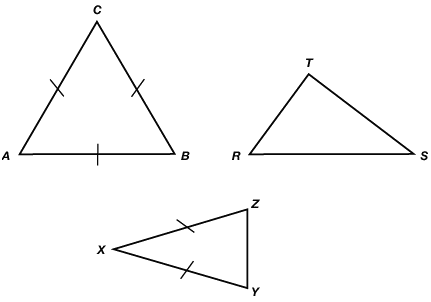
\includegraphics[scale=.5]{teste-de-software/conceitos-basicos/Imagens/triangulo-equilatero-isosceles-escaleno}}
\end{block}
\end{frame}


\begin{frame}[hasprev=true, hasnext=false]
\frametitle{Falhas}

\begin{block:fact}{Evitar e detectar falhas}
\begin{itemize}
	\item No entanto, produtos com falhas podem e devem ser evitados e corrigidos, uma vez que afeta negativamente a qualidade do software
\end{itemize}
\end{block:fact}


\begin{block:fact}{Por que devemos nos preocupar com isso?}
\begin{itemize}
    \item A crescente demanda por maior qualidade de software

    \item A redução de falhas no software melhora sua qualidade.
\end{itemize}
\end{block:fact}

\begin{block:fact}{Qualidade e teste de software}
\begin{itemize}
	\item O principal objetivo do teste de software é encontrar falhas.

	\item Testes de softwares sistemáticos, realizada utilizando técnicas adequadas, critérios e ferramentas, melhora a confiabilidade do software (e qualidade).
\end{itemize}
\end{block:fact}
\end{frame}

 
 \section{Teste de software}
 \begin{frame}[parent={cmap:software-testing-foundations}, hasprev=false, hasnext=true]
\frametitle{Teste de software}

\begin{block:fact}{Motivação}
\begin{itemize}
	\item Software contém falhas.

	\item Testar o software pode revelar várias falhas.
\end{itemize}
\end{block:fact}

\begin{block:fact}{Teste de software como uma disciplina}
\begin{itemize}
	\item Teste \textit{Ad hoc} é insuficiente e ineficaz na detecção de falhas.
	\begin{itemize}
		\item É difícil pensar em casos de testes o suficiente até mesmo para software simples.
		(como o triângulo).
	\end{itemize}

	\item O teste de software deve ser tomado como uma disciplina
	\begin{itemize}
		\item Os casos de teste devem ser criados para avaliar a qualidade dos artefatos do software (principalmente a especificação de requisitos e o código-fonte) em relação aos critérios estabelecidos.

		\item As técnicas devem ser desenvolvidas para detectar o máximo de falhas possíveis no software.
	\end{itemize}
\end{itemize}
\end{block:fact}
\end{frame}


\begin{frame}[hasprev=true, hasnext=true]
\frametitle{Teste de software}
\framesubtitle{Definição}
\label{concept:teste-de-software}

\begin{block:concept}{Definição}
O teste de software é o processo de operação de um sistema ou componente em condições especificadas, observando ou registrando os resultados, e fazendo uma avaliação de alguns aspectos do sistema ou componente~\cite{ieee610.12:1990}.
\end{block:concept}

\begin{block:fact}{Teste de software é\dots{}}
\begin{itemize}
	\item uma atividade de verificação e validação,

	\item importante para a manutenção, avaliação da confiabilidade, melhoria de processos de software, depuração,

	\item uma atividade dinâmica,
	\begin{itemize}
		\item Isso requer a execução do programa (análise estática não é suficiente),
	\end{itemize}

	\item custoso~\cite{harrold:2000}
\end{itemize}
\end{block:fact}
\end{frame}



\begin{frame}
\frametitle{Teste de software}
\framesubtitle{Objetivo}

\begin{block:fact}{Objetivo}
\begin{itemize}
	\item O objetivo do teste de software é detectar falhas no produto em fase de testes.
\end{itemize}
\end{block:fact}

\begin{block:fact}{}
Primeiro erro já detectado (por Grace Hopper). É um bug real (é por isso que chamamos erro de bug até hoje).
\centering
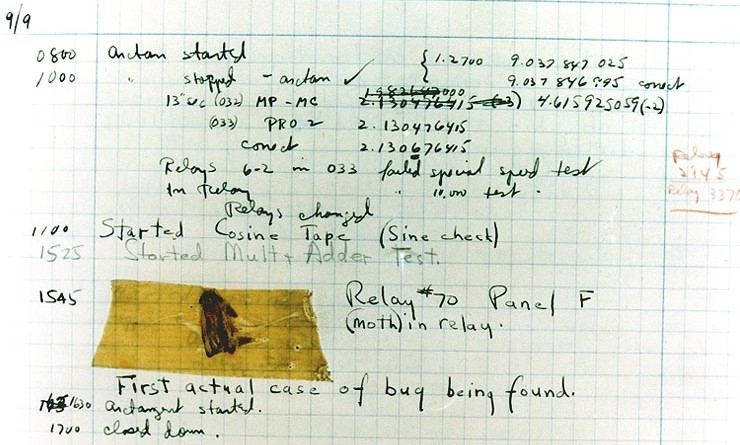
\includegraphics[width=7cm]{teste-de-software/conceitos-basicos/Imagens/first-bug}
\end{block:fact}
\end{frame}


\begin{frame}
\frametitle{Teste de software}
\framesubtitle{Análise racional}

\begin{block:fact}{Contradição}
\begin{itemize}
	\item Assim, testes de software visa apenas destruir o software?
	\begin{itemize}
		\item Afinal de contas, o programador gasta horas implementando-o e as atividades de teste encontrarão erros no trabalho feito por ele
	\end{itemize}
\end{itemize}
\end{block:fact}

\begin{block:fact}{Análise relacional}
\begin{itemize}
	\item Humans are highly goal-oriented (and proper goals has an important
	psychological effect~\cite[p. 6]{myers:2004}).

	\item Se o objetivo é demonstrar que o programa não tem nenhum erro, então o dispositivo de teste subconscientemente será conduzido em direção a esse objetivo.
	\begin{itemize}
		\item Haverá uma tendência para selecionar dados que possuem uma baixa probabilidade de causar falhas nos programas.
	\end{itemize}

	\item Se o objetivo é demonstrar que o programa tem falhas, os casos de teste terão uma maior probabilidade de encontrar os erros.
\end{itemize}
\end{block:fact}
\end{frame}



\begin{frame}
\frametitle{Teste de software}
\framesubtitle{Análise relacional}

\begin{block:principle}{Análise relacional}
O processo de demonstração de que os erros não estão presentes é impossível de alcançar virtualmente todos os programas (mesmo os triviais).
\end{block:principle}

\begin{block:fact}{Problemas indertemináveis}
\begin{itemize}
	\item A avaliação de correção de um programa é um problema indeterminável.
	\begin{itemize}
		\item Indeterminado = não computável.
	\end{itemize}

	\item Os erros podem ser camuflados por outros erros devido a correções coincidentes.
	\begin{itemize}
		\item A avaliação de correção coincidente também é um problema inderterminável.
	\end{itemize}

	\item Several other undecidable problems plague (praga, aplicáveis) software testing: software
	equivalence, executability.
\end{itemize}
\end{block:fact}
\end{frame}


\begin{frame}
\frametitle{Teste de software}
\framesubtitle{Conceitos principais}

\begin{block:fact}{Como são detectadas as falhas?}
\begin{itemize}
	\item As falhas são detectadas através da execução do software contra um conjunto de casos de teste.
\end{itemize}
\end{block:fact}

\begin{block:procedure}{Execução do caso de teste}
\begin{enumerate}
	\item Definir os dados de entrada que serão fornecidos ao software sob teste.

	\item Execute o software.

	\item Checar se os resultados das produção do software era o esperado (para os dados de entrada fornecido)
	\begin{itemize}
		\item Se o resultado é correto, mantenha a definição de diferentes casos de entrada.

		\item Se o resultado é incorreto, uma falha foi encontrada! Sucesso!
	\end{itemize}
\end{enumerate}
\end{block:procedure}
\end{frame}



\begin{frame}
\frametitle{Teste de software}
\framesubtitle{Conceitos principais}

\begin{block:principle}{Teste exaustivo}
Se o software é executado com todos os dados possíveis, qualquer falha será encontrada
\end{block:principle}

\begin{block:fact}{Viabilidade e computabilidade}
Infelizmente, muitas vezes não é possível executar testes exaustivamente devido a alguns problemas computacionais:
\begin{itemize}
	\item O dados de entrada podem ser tão grandes que é impossível executar o software com ele em um tempo razoável;

	\item Computabilidade (problemas indertemináveis).
\end{itemize}
\end{block:fact}
\end{frame}


\begin{frame}
\frametitle{Teste de software}
\framesubtitle{Conceitos principais}

\begin{block:principle}{Divisão de domínio}
No entanto, é possível particionar o domínio de entrada e, em vez de usar todos os elementos dentro de cada partição, apenas poucas entradas são selecionadas (e aceito como uma boa representação de cada elemento do conjunto).
\end{block:principle}

\begin{block:fact}{Técnicas e critérios}
\begin{itemize}
	\item Critérios de teste definem as regras a respeito de como um determinado dado de entrada é dividido;

	\item Tais regras, quando aplicado ao software sob teste, gera necessidade de teste:
	\begin{itemize}
		\item Requisitos de teste é uma combinação de elementos do programa com os testes devem ser satisfeitas pela execução de um caso de teste.
	\end{itemize}

	\item Técnicas de teste definem a razão e a fonte de informação que orienta o desenvolvimento de critérios de teste.
\end{itemize}
\end{block:fact}
\end{frame}




\begin{frame}[c, hasprev=true, hasnext=false]
\frametitle{Teste de software concepts}
\framesubtitle{Conceitos principais}

\begin{block:fact}{}
	\centering
	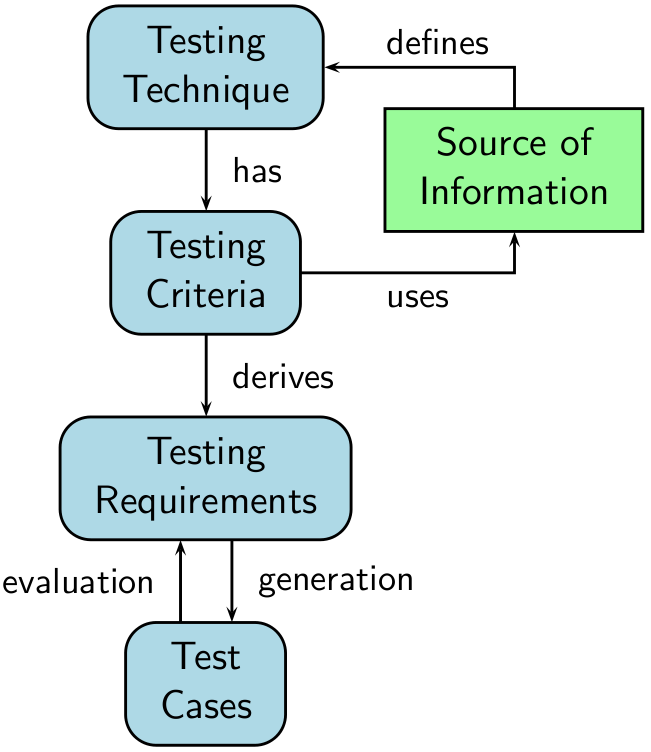
\includegraphics[scale=.3]{teste-de-software/conceitos-basicos/Imagens/software-testing}
\end{block:fact}
\end{frame}
 
 \section{Erro de taxonomia}
 \begin{frame}[parent={cmap:software-testing-foundations}, hasprev=false, hasnext=true]
\frametitle{Erro de taxonomia}
\framesubtitle{Falhas}
\label{concept:fault}

\begin{block:concept}{O que é uma falha?}
Uma falha é uma definição de dados, passos ou processos incorretos em um software. 
\end{block:concept}

\begin{block:fact}{Como uma falha é criado?}
\begin{itemize}
	\item Uma falha é inserido por um erro.
\end{itemize}
\end{block:fact}

\hfill
\refie{example:incorrect-statement-2}{\beamerbutton{Example: Declaração incorreta}}
\end{frame}



\begin{frame}[hasprev=true, hasnext=true]
\label{concept:mistake}
\frametitle{Erro de taxonomia}
\framesubtitle{Erro}

\begin{block:concept}{O que é um erro?}
Um erro é uma ação humana que produz um resultado incorreto.
\end{block:concept}

\begin{block:fact}{Como um erro ocorre?}
\begin{itemize}
	\item Pela falta de atenção durante a execução de um software?

	\item Pela omissão de informações na especificação de requisitos do software?

	\item Erro de compilação (ocasionado por um erro)?
\end{itemize}
\end{block:fact}

\hfill
\refie{example:incorrect-statement-1}{\beamerbutton{Example: Declaração incorreta}}
\end{frame}



\begin{frame}
\label{concept:error}
\frametitle{Erro de taxonomia}
\framesubtitle{Error}

\begin{block:concept}{O que é um erro?}
An error is the difference between a computed, observed or measured value
or condition and the true, theoretically correct or specified value or
condition.
\end{block:concept}

\begin{block:fact}{Como um erro ocorre?}
\begin{itemize}
	\item Um erro é produzido pela execução de uma falha.
	\begin{itemize}
		\item Assim, se uma falha nunca é executada, ele nunca produz um erro.
	\end{itemize}
\end{itemize}
\end{block:fact}
\end{frame}


\begin{frame}
\label{concept:failure}
\frametitle{Erro de taxonomia}
\framesubtitle{Falha}

\begin{block:concept}{O que é uma falha?}
Uma falha é a incapacidade de um componente ou um sistema de cumprir suas funções necessárias dentro dos requisitos de desempenho especificados.
\end{block:concept}

\begin{block:fact}{Como uma falha ocorre?}
\begin{itemize}
	\item Uma falha e seus erros associados podem causar uma ou mais falhas.
\end{itemize}
\end{block:fact}

\hfill
\refie{example:incorrect-statement-3}{\beamerbutton{Example: Declaração incorreta}}
\end{frame}



\begin{frame}
\frametitle{Erro de taxonomia}

\begin{block:procedure}{Summary}
\begin{enumerate}
	\item Um programador comete um \textbf{erro}.
	\begin{itemize}
		\item Um único $<$ passa a ter um $>$ em uma única instrução.
	\end{itemize}

	\item Devido ao erro, a declaração está com \textbf{falha} (não implementar o comportamento descrito na especificação de requisitos de software).

	\item O software é compilado e executado. A instrução fornecida é executada. Como ele pertence a uma função responsável pela criação da soma de verificação dos dados que estão sendo processados, a saída que é produzida é incorreta (\textbf{erro}).

	\item O usuário compara a soma de verificação produzido pelo software com o resultado esperado. Não importa o que, a soma de verificação sempre \textbf{falha}.
\end{enumerate}
\end{block:procedure}
\end{frame}



\begin{frame}[c, hasprev=true, hasnext=false]
\label{concept:defect-taxonomy}
\frametitle{Erro de taxonomia}

\begin{block:fact}{}
    \centering
    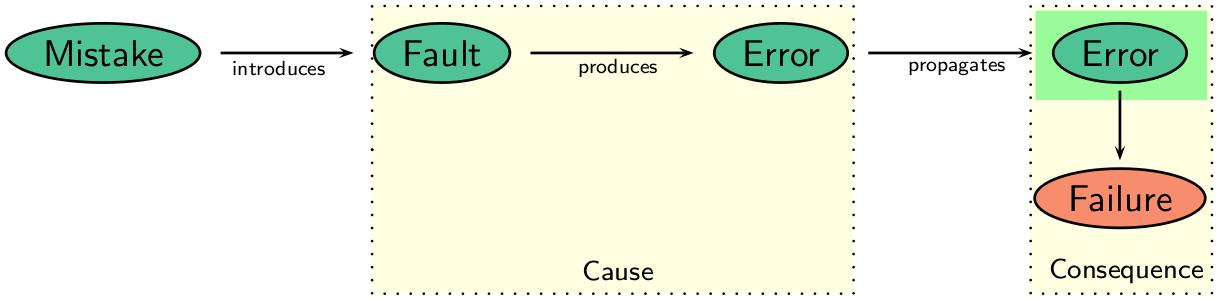
\includegraphics[scale=.3]{teste-de-software/conceitos-basicos/Imagens/defect-taxonomy}
\end{block:fact}

\hfill
\refie{example:physician-analogy-for-defect-taxonomy}{\beamerbutton{Example: Physician analogy for defect taxonomy}}
\refie{example:numzero}{\beamerbutton{Example: Exemplo de erro de taxonomia (numZero)}}
\end{frame}

 
 \section{Casos de teste}
 \begin{frame}[parent={cmap:software-testing-foundations}, hasprev=false, hasnext=true]
\frametitle{Casos de teste}
\label{concept:test-case}
\label{concept:input-domain}
\label{concept:output-domain}
\label{concept:input-data}
\label{concept:output-data}

\begin{block:concept}{Definição simplificada}
Um caso de teste é constituído de um par de dados de teste (um conjunto de valores, um para cada variável) para ser os dados de entrada do programa e o resultado esperado.
\end{block:concept}


\begin{block:concept}{A melhor definição}
Um caso de teste é geralmente definido como uma tupla $(d, S(d))$, onde:
\begin{itemize}
	\item $d \in D$ (e $D$ é conjunto de entrada), e;
	\item $S(d)$ representa o resultado esperado para a entrada $d$ de acordo com a especificação $S$.
\end{itemize}
\end{block:concept}

\hfill
\refie{example:sort-test-cases}{\beamerbutton{Example: Casos de teste para um método de ordenação}}
\refie{example:num-zero-test-cases}{\beamerbutton{Example: Casos de teste para o método numZero}}
\end{frame}


\begin{frame}[hasprev=false, hasnext=true]
\frametitle{Casos de teste}
\framesubtitle{Assessing a test case}
\label{concept:test-case-success}
\label{concept:test-case-failure}

\begin{block:fact}{Casos de teste de sucesso}
\begin{itemize}
	\item Primeiro, um caso de teste bem-construido e executado é bem sucedida quando encontra erros.~\cite[p. 7]{myers:2004}

	\item Ele também é bem sucedido quando estabelece eventualmente que não há mais erros que podem ser encontrados (como quando se aplica um critério de teste e satisfaz todos os requitido de teste).
\end{itemize}
\end{block:fact}

\begin{block:fact}{Casos de teste sem sucesso}
\begin{itemize}
	\item Um caso de teste sem sucesso é aquele que faz com que um programa chegue ao resultado correto sem encontrar nenhum erro.
\end{itemize}
\end{block:fact}

\hfill
\refie{example:doctor-laboratory-test}{\beamerbutton{Analogia para casos de teste eficientes e ineficientes}}
\end{frame}



\begin{frame}
\frametitle{Casos de teste}

\begin{block:fact}{Ordem de execução}
\begin{itemize}
    \item Há dois tipos de casos de teste em relação a ordem de execução do teste:
	\begin{itemize}
		\item Caso de teste sequencial, e;
		\item Caso de teste independete.
	\end{itemize}
\end{itemize}
\end{block:fact}
\end{frame}


\begin{frame}
\label{concept:cascading-test-case}
\frametitle{Casos de teste}
\framesubtitle{Caso de teste sequencial}

\begin{block:concept}{Definição}
Casos de teste sequenciais são casos de testes que dependem uns dos outros.
\end{block:concept}


\begin{block:fact}{Vantagens e disvantagens}
\begin{itemize}
	\item A vantagem dos casos de teste sequencial é que cada caso de teste é normalmente pequeno e simples;

	\item A disvatagem dos casos de teste sequencial é que se um teste falha, os testes subsequentes podem ser inválidos.
\end{itemize}
\end{block:fact}

\hfill
\refie{example:cascading-test-case}{\beamerbutton{Example: Casos de teste sequencial}}
\end{frame}



\begin{frame}[hasprev=true, hasnext=false]
\label{concept:independent-test-case}
\frametitle{Casos de teste}
\framesubtitle{Casos de teste independentes}

\begin{block:concept}{Definição}
Casos de teste independentes são totalmente autônomos.
\begin{itemize}
	\item Casos de teste independentes não dependem uns dos outros, nem exigir que outros testes fossem executado com sucesso.
\end{itemize}
\end{block:concept}

\begin{block:fact}{Vantagens e disvantagens}
\begin{itemize}
	\item A vantagem dos casos de teste independentes é que qualquer número de testes pode ser executado em qualquer ordem;

	\item A disvantagem dos casos de teste independentesque cada teste tende a ser maior e mais complexo e, portanto, mais difícil de criar, projetar e manter.
\end{itemize}
\end{block:fact}
\end{frame}
 
 \section{Oráculo}
 \begin{frame}[parent={cmap:software-testing-foundations}, hasprev=false, hasnext=true]
\frametitle{Oráculo}

\begin{block:fact}{Está correto?}
\begin{itemize}
	\item Dado um conjunto de condições de entrada e as observações do resultado computacional, quem decide qual é o resultado correto?

	\item Alguém ou alguma coisa deve verificar se o software, para um determinado caso de teste, tem funcionado corretamente.
\end{itemize}
\end{block:fact}
\end{frame}


\begin{frame}[hasprev=true, hasnext=true]
\frametitle{Oráculo}
\label{concept:oracle}

\begin{block:concept}{Definição}
Um oráculo é qualquer software, processo or dado que fornece o gerador de provas com o resultado esperado de cada caso de teste.
\end{block:concept}

\begin{block:fact}{}
\begin{itemize}
	\item Um oráculo decide se os valores de saída estão correto de acordo com o está especificado.
	\begin{itemize}
		\item Um oráculo é necessário para determinar se a falha foi revelada.
	\end{itemize}

	% TODO: Propose a better classification of oráculos
	\item Alguns exemplos de oráculo: suposição humana (kiddie oráculo), conjunto de teste de regressão, dados avaliados, conjunto de teste adquirido, software existente.
\end{itemize}
\end{block:fact}
\end{frame}



\begin{frame}
\label{concept:kiddie-oracle}
\frametitle{Oráculo}
\framesubtitle{Kiddie oráculo}

\begin{block:concept}{Definição}
A kiddie oráculo é obtido a partir de executar o software e ver a saída. Se ele se parece com o da direita, ele deve estar certo.
\end{block:concept}

\begin{block:fact}{Por que eu deveria usar um kiddie oráculo?}
\begin{itemize}
	\item Na verdade, você não deve usá-lo, pois é sujeito a erros;

	\item Entretanto, é melhor do que anda.
	\begin{itemize}
		\item E, se o comportamento esperado da aplicação não está documentada, é de responsabilidade do usuário detectar o resultado correto de qualquer maneira.
	\end{itemize}
\end{itemize}
\end{block:fact}

\hfill
\refie{example:kiddie-oráculo}{\beamerbutton{Example: Human guess (kiddie) oráculo}}
\end{frame}



\begin{frame}
\label{concept:regression-test-suite-oracle}
\frametitle{Oráculo}
\framesubtitle{Regression test suite oráculo}

\begin{block:concept}{Definição}
A regression test suite oráculo  is obtained from running the test case and
comparing the output to the results of the same test cases run against a
previous version of the software.
\end{block:concept}

\begin{block:fact}{Why should I use a regression suite oráculo?}
\begin{itemize}
	\item Regression test ensures that the modified system functions as per
	its specification.

	\item It ensures that old errors will not appear again (or that, at least,
	they will be early detected).
\end{itemize}
\end{block:fact}

\hfill
\refie{example:mozilla-firefox-regression-test-suite-oráculo}{\beamerbutton{Example: Regression test suite oráculo for Mozilla Firefox}}
\end{frame}



\begin{frame}[hasprev=true, hasnext=false]
\label{concept:purchased-test-suite-oracle}
\frametitle{Oráculo}
\framesubtitle{Aquisição do suite de teste oráculo}

\begin{block:concept}{Definição}
Uma compra do suite de teste oráculo consiste em executar o software com uma série de testes normalizados que tenha sido previavemente criado e validado.
\end{block:concept}

\begin{block:fact}{Por que eu deveria usar um oráculo com}
\begin{itemize}
	\item Normalmente é necessário que um software passe um conjunto de testes oráculo, com a finalidade de avaliar a sua conformidade com uma específica tecnologia ou padrão;

	\item As vezes, é simplesmente mais fácil comprar um conjunto de testes a desenvolver seu próprio conjunto de testes.
\end{itemize}
\end{block:fact}


\hfill
\refie{example:java-test-suite-oráculo}{\beamerbutton{Example: Java TCK}}
\end{frame}
 
 \section{Fase de teste}
 \begin{frame}[parent={cmap:software-testing-foundations}, hasprev=false, hasnext=true]
\frametitle{Fases de teste}

\begin{block:fact}{O que devo testar primeiro?}
\begin{itemize}
	\item O que devo direcionar ao teste de software?

	\item A definição de um único alvo para cada atividade de teste é fundamental para teste de software sistemático.
	\begin{itemize}
		\item Fono na aplicação e restrição de técnicas disponíveis (diminuindo assim os custose, provavelmente, aumentando a eficácia).
	\end{itemize}

	\item Uma abordagem de senso comum seria iniciar o teste com a menor função possível, e depois prosseguir para testar as interações entre as funções e, finalmente, o sistema como um todo.
\end{itemize}
\end{block:fact}
\end{frame}


\begin{frame}[hasprev=true, hasnext=true]
\frametitle{Fases de teste}
\label{concept:test-phase}
\label{concept:phase}

\begin{block:concept}{Definição}
A fase de teste é uma categorização da atividade de teste que está diretamente relacionada com o ciclo de vida do software e as atividades que acontecem no software.
\end{block:concept}

\begin{block:fact}{Definições}
\begin{itemize}
	\item Fases de teste permite que o dispositivo de teste se concentre em vários aspectos do software e utilize diferentes critérios de teste para cada um;

	\item As atividades de teste são organizadas em fases de teste de modo que o teste inicie com a menor unidade executável até alcançar o software como um todo:
	\begin{itemize}
		\item Teste de unidade;
		\item Teste de integração;
		\item Teste do sitema;
		\item Teste de aceitação.
	\end{itemize}
\end{itemize}
\end{block:fact}
\end{frame}


\begin{frame}[c]
\frametitle{Fases de teste}

\begin{block:fact}{}
    \centering
    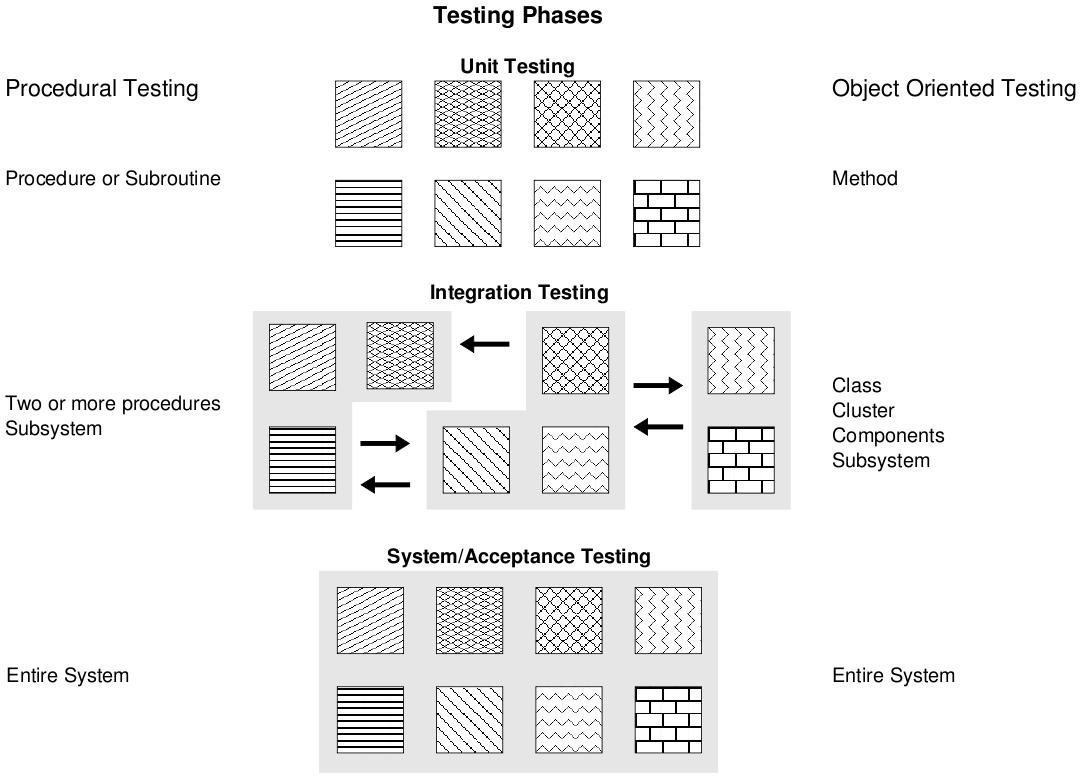
\includegraphics[scale=.3]{teste-de-software/conceitos-basicos/Imagens/fases-de-teste}
\end{block:fact}
\end{frame}


\begin{frame}
\frametitle{Fases de teste}
\framesubtitle{Teste de unidade}
\label{concept:unit-testing}

\begin{block:concept}{Definição}
Teste de unidade verifica o funcionamento isolado de fragmentos do software que são testados separadamente.
\end{block:concept}

\begin{block:fact}{}
    \centering
    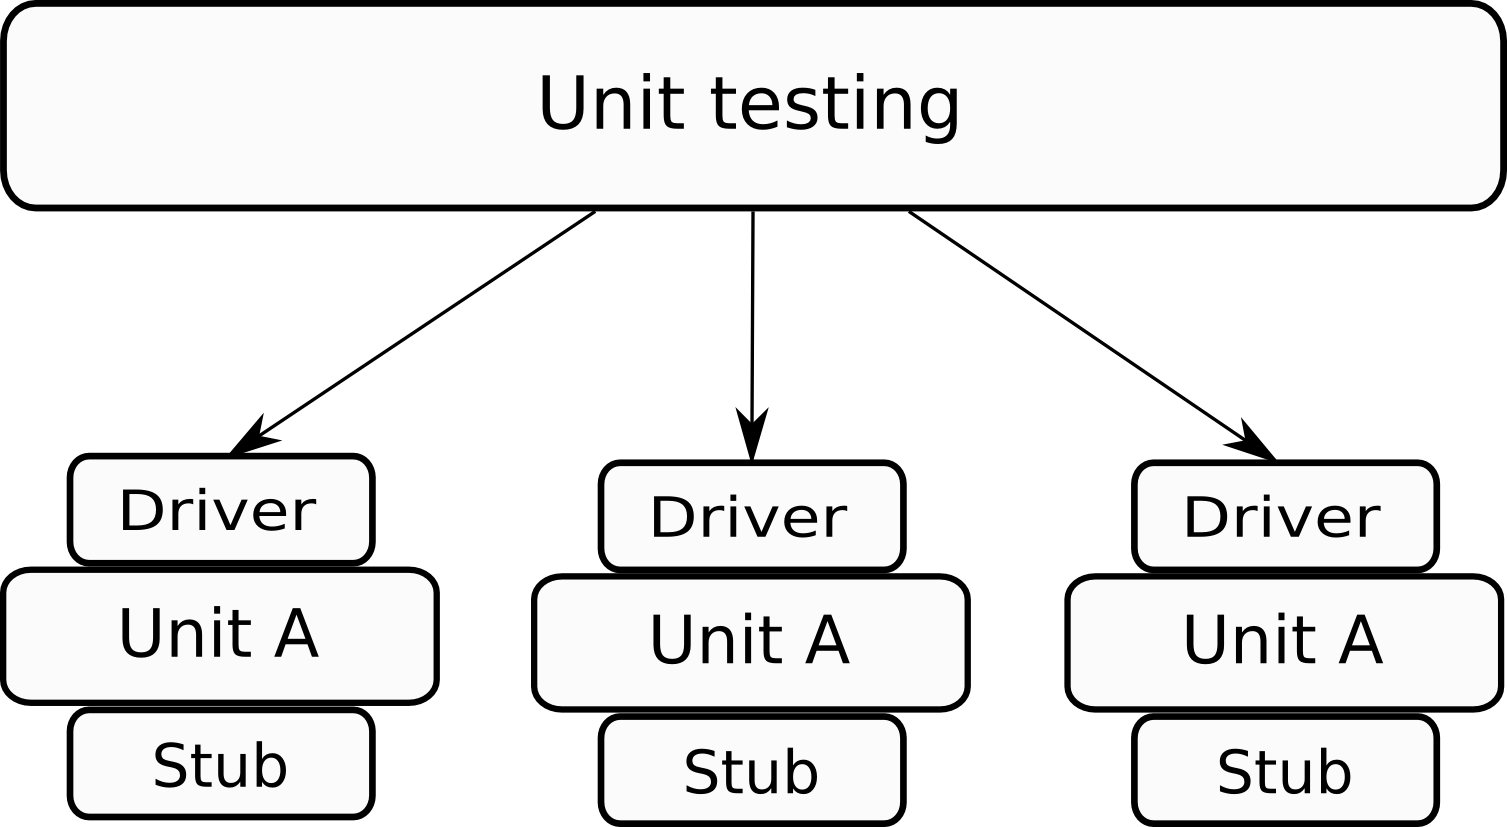
\includegraphics[width=5cm]{teste-de-software/conceitos-basicos/Imagens/teste-unitario}
\end{block:fact}

\hfill
\refie{example:pentium-fdiv-bug}{\beamerbutton{Example: Pentium FDIV bug}}
\end{frame}


\begin{frame}
\frametitle{Fases de teste}
\framesubtitle{Teste de unidade}

\begin{block:fact}{O que é uma unidade?}
\begin{itemize}
	\item Em teste de processo, a unidade é o procedimento ou a subrotina;

	\item Em teste orientado a objeto, a unidade é um método ou uma classe:
	\begin{itemize}
		\item Por enquanto, vamos considerar que a unidade é um método.
	\end{itemize}
\end{itemize}
\end{block:fact}
\end{frame}



\begin{frame}
\frametitle{Fases de teste}
\framesubtitle{Teste de unidade - Stubs}
  
\begin{block:fact}{Como testar uma unidade?}
\begin{itemize}
	\item Embora a definição diz para testar as unidades separademente, nem sempre isso é possível:
	\begin{itemize}
		\item Muitas unidade necessitam de dados de outras unidade.
	\end{itemize}

	\item A ligação entre os métodos é uma ameaça para o teste unitário. Assim, é desejável substituir algumas unidades por outras mais simples e previsíveis (apenas para o fim do teste de software).
\end{itemize}
\end{block:fact}
\end{frame}



\begin{frame}
\frametitle{Fases de teste}
\framesubtitle{Stubs}
\label{concept:stub}

\begin{block:concept}{Definição}
Um stub é uma unidade que substitui outra unidade utilizada pela unidade em teste.
\end{block:concept}

\begin{block:fact}{Por que devemos usar um stub?}
\begin{itemize}
	\item Stubs simula o comportamento de outra unida que ainda não foi implementado, mas foi chamado pela unidade em teste.

	\item Geralmente, um stub simula o comportamento esperado da unidade utilizada com o mínimo de esforço computacional possível ou manipulação de dados.
\end{itemize}
\end{block:fact}

\hfill
\refie{example:stub}{\beamerbutton{Example: Stub}}
\end{frame}


\begin{frame}
\frametitle{Fases de teste}
\framesubtitle{Teste de unidade - Driver}

\begin{block:fact}{Como testar uma unidade?}
\begin{itemize}
	\item Mesmo que stubs pode ser usado para substituir unidades complexas para uma determinada unidade em fase de testes 
\end{itemize}
\end{block:fact}
\end{frame}



\begin{frame}
\frametitle{Fases de teste}
\framesubtitle{Teste de unidade - Driver}
\label{concept:driver}
\label{concept:test-driver}

\begin{block:concept}{Definição}
Driver é o software responsável por coordenar o teste de uma unidade.
\end{block:concept}

\begin{block:fact}{O que um driver faz?}
\begin{itemize}
	\item Drivers são usados para testar uma unidade que requer dados de entrada fornecidos por outra unidade:
	\begin{enumerate}
		\item Reúne os dados fornecidos pelo verificador;
		\item É passado para a unidade em teste na forma de argumentos;
		\item Que recolhe os resultados produzidos pela unidade, e;
		\item Mostra todos eles para o verificador.
	\end{enumerate}
\end{itemize}
\end{block:fact}
\end{frame}


\begin{frame}[c]
\frametitle{Fases de teste}
\framesubtitle{Teste de unidade - Driver and stubs}

\begin{block:fact}{}
	\centering
	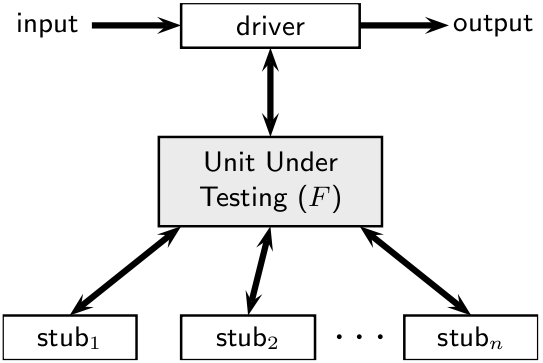
\includegraphics[scale=.3]{teste-de-software/conceitos-basicos/Imagens/driver-e-stub}
\end{block:fact}
\end{frame}



\begin{frame}
\label{concept:integration-testing}
\frametitle{Fases de teste}
\framesubtitle{Teste de integração}

\begin{block:concept}{Definição}
Teste de integridade verifica se as variáveis testadas individualmente se comunicam corretamente quando integrado.
\end{block:concept}

\begin{block:fact}{}
    \centering
    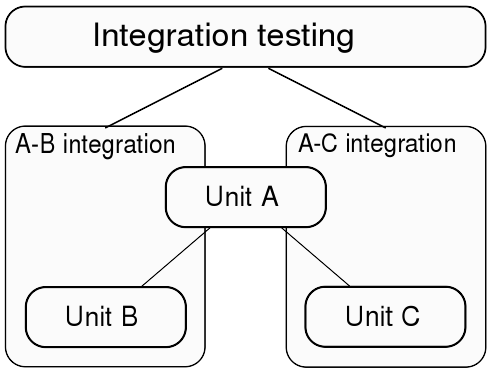
\includegraphics[scale=.3]{teste-de-software/conceitos-basicos/Imagens/integration-testing}
\end{block:fact}

\hfill
\refie{example:mars-climate-orbiter}{\beamerbutton{Example: Mars climate orbiter}}
\end{frame}



\begin{frame}
\frametitle{Fases de teste}
\framesubtitle{Teste de integridade}

\begin{block:fact}{Por que o teste de integração é importante?}
\begin{itemize}
	\item Teste de integridade deve ser executado porque:
	\begin{itemize}
		\item Os dados podem ser perdidos na interfáce da variável;

		\item Variáveis globais podem sofrer interferências indesejadas.
	\end{itemize}
\end{itemize}
\end{block:fact}

\begin{block:fact}{}
    \centering
    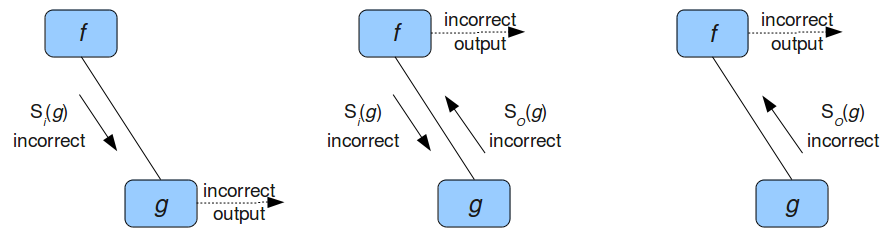
\includegraphics[width=\textwidth]{teste-de-software/conceitos-basicos/Imagens/types-integration-errors}
\end{block:fact}
\end{frame}


\begin{frame}
\label{concept:system-testing}
\frametitle{Fases de teste}
\framesubtitle{Teste de sistema}

\begin{block:concept}{Definição}
Teste de sistema garante que o software e os outros elementos que fazem parte do sistema (hardware e banco de dados, por exempo) são combinados adequadamente e se comportam conforme o esperado.
\end{block:concept}

\begin{block:fact}{Tipos de teste de sistema}
\begin{itemize}
	\item Normalmente o teste de sistema inclui muitos tipos de teste
	\begin{columns}[t, totalwidth=6.5cm]
		\begin{column}[t]{3cm}
			\begin{itemize}
				\item Funcionalidade;,
				\item Usabilidade;
				\item Segurança;
				\item Localização.
			\end{itemize}
		\end{column}

		\begin{column}[t]{3cm}
			\begin{itemize}
				\item Confiabilidade;
				\item Disponibilidade.
				\item \ldots
			\end{itemize}
		\end{column}
	\end{columns}
\end{itemize}
\end{block:fact}

\hfill
\refie{example:trem-fantasma}{\beamerbutton{Example: Trem fantasma}}
\end{frame}



\begin{frame}[hasprev=true, hasnext=false]
\label{concept:acceptance-testing}
\frametitle{Fases de teste}
\framesubtitle{Teste de aceitação}

\begin{block:concept}{Definição}
Teste de aceitação refere-se ao avaliador, geralmente realizado pelo próprio usuário que verifica se o produto satisfaz sua expectativa.
\end{block:concept}

\begin{block:fact}{Teste Alfa/Beta}
\begin{itemize}
	\item Informalmente, pode ser definido como teste alfa e beta:
	\begin{itemize}
		\item Teste alfa: o software é instalado e usado internamente (na em presa em que foi desenvolvida);

		\item Teste beta: o software é instalado e testado por usuários exeternos.
	\end{itemize}
\end{itemize}
\end{block:fact}

\begin{block:fact}{Por que o teste de aceitação é importante?}
\begin{itemize}
    \item O teste de aceitação, quando concluído com sucesso, resultará na aceitação do software pelo cliente.
\end{itemize}
\end{block:fact}
\end{frame}
 
 \section{Teste de critérios}
 \begin{frame}[parent={cmap:software-testing-foundations}, hasprev=false, hasnext=true]
\frametitle{Critério de teste}

\begin{block:fact}{Técnicas e critérios de teste}
\begin{itemize}
	\item Técnicas de teste fornece uma teoria fundamentada de como devemos testar nosso software:
	\begin{itemize}
		\item Quais são as fontes de requisito de teste?

		\item Quais as características das fontes devem ser exploradas?
	\end{itemize}

	\item Entretanto, a fim de testar um software com sucesso, deve ser cuidadosamente especificada como deve ser aplicado as técnicas.
	\begin{itemize}
		\item Queremos dizer com êxito: encontrar erros.
	\end{itemize}
\end{itemize}
\end{block:fact}


\begin{block:fact}{Como aumentar a eficiência}
\begin{itemize}
	\item {\small Os requisitos de teste deve ser estabelecido para explorar não só o que o software deve fazer, mas também o que ele \textbf{não} deve fazer;}

	\item {\small Uma medida também deve ser fornecida, de modo que um critério de parada possa ser definido para o teste de atividade.}
\end{itemize}
\end{block:fact}
\end{frame}



\begin{frame}[hasprev=true, hasnext=true]
\label{concept:test-criterion}
\frametitle{Critério de teste}

\begin{block:concept}{Definição}
Um critério de teste sistematiza a forma que os requisitos de teste são gerados a partir da fonte de informação(especificação, código fonte, histórico de falhas do banco de dados).
\end{block:concept}

\begin{block:fact}{}
\begin{itemize}
	\item Um critérios de teste fornece uma forma sistemática para selecionar os casos de teste:
	\begin{itemize}
		\item Um critério de teste divide as entradas.
	\end{itemize}

	\item Quando não há falhas encontradas, o critério de teste fornece uma indicação de como os casos de testes devem ser selecionados a fim de estabelecer um alto nível de de confiança de correção do produto.
\end{itemize}
\end{block:fact}


\hfill
\refie{example:test-criterion}{\beamerbutton{Example: Critério de teste example}}
\end{frame}


\begin{frame}
\frametitle{Critério de teste}

\begin{block:fact}{Critério de teste attributes}
\begin{itemize}
	\item Um critério de teste pode ser comparado baseado no custo, eficácia e resistência.
\end{itemize}
\end{block:fact}

\begin{block:fact}{}
    \centering
    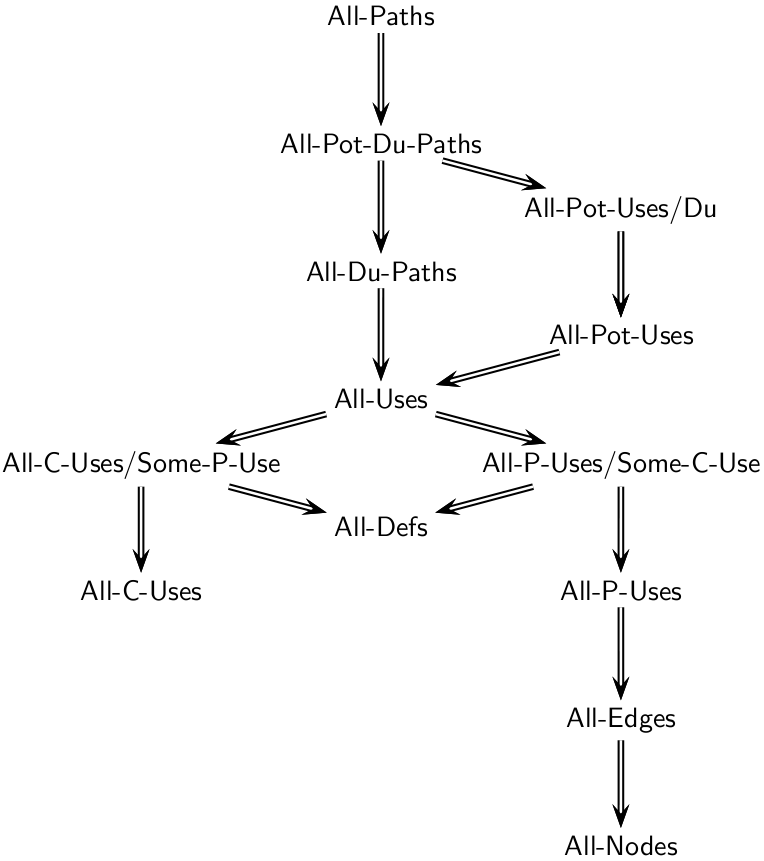
\includegraphics[width=4cm]{teste-de-software/conceitos-basicos/Imagens/subsume-relation}
\end{block:fact}
\end{frame}


\begin{frame}[hasprev=true, hasnext=false]
\frametitle{Critério de teste}

\begin{block:fact}{Teste de cobertura}
\begin{itemize}
	\item Um teste de critério pode ser usado tanto para avaliar o programa em fase de teste ou para avaliação de consistência de um conjunto de teste.
\end{itemize}
\end{block:fact}

\begin{block:concept}{Teste de seleção de critério}
O teste de critério é usado para selecionar casos de teste que avaliem o programa em fase de teste.
\end{block:concept}


\begin{block:concept}{Teste de avaliação de critério}
O teste de critério é utilizado para avaliar os conjuntos de teste.
\end{block:concept}
\end{frame}


% Test cases representing unexpected and invalid input conditions seem to
% have a higher error-detection yield than do test cases for valid input
% conditions~\cite[p. 18]{myers:2004}.
% \begin{itemize}
%	\item Programs must be examined for unwanted side effects~\cite[p. 18]{myers:2004}.
% \end{itemize}


 
 \section{Teste de requisitos}
 \begin{frame}[parent={cmap:software-testing-foundations}, hasprev=false, hasnext=true]
\frametitle{Requisito de teste}
\label{concept:test-requirement}

\begin{block:concept}{Definição}
O requisito de teste é um elemento especificado de um artefato do software que um caso de teste deve satisfazer ou cobrir.
\end{block:concept}

\begin{block:fact}{Como um teste de requisito é criado?}
\begin{itemize}
	\item Os requisitos de teste são derivados do programa em teste usando um critério de teste específico.
\end{itemize}
\end{block:fact}

\begin{block:fact}{Para que servem os requisitos de teste?}
\begin{itemize}
	\item O requisito de teste pode:
	\begin{itemize}
		\item avaliar um conjunto de teste, e;
		\item gerar um conjunto de teste.
	\end{itemize}
\end{itemize}
\end{block:fact}
\end{frame}


\begin{frame}[hasprev=true, hasnext=false]
\label{concept:test-set}
\label{concept:c-adequate-test-set}
\frametitle{Requisito de teste}
\framesubtitle{Conjunto de teste}

\begin{block:concept}{Definição}
Um conjunto de teste é um conjunto de casos de teste.
\end{block:concept}

\begin{block:fact}{Conjunto de testes e requisitos de teste}
\begin{itemize}
	\item Um conjunto de teste pode ser melhorado pela adição de casos de teste que buscam requisitos a serem descobertos.
	\begin{itemize}
		\item O melhor conjunto de teste é o menor que indica o maior conjunto de erros.
	\end{itemize}
\end{itemize}
\end{block:fact}

\begin{block:concept}{C-adequate test sets}
\begin{itemize}
	\item Quando um conjunto de teste $T$ satisfaz todos os requisitos de teste derivado de um programa utilizando dados os critérios $C$, $T$ diz $C-adequado$.
\end{itemize}
\end{block:concept}
\end{frame}

 \section{Técnicas de teste}
 \begin{frame}[parent={cmap:software-testing-foundations}, hasprev=false, hasnext=true]
\frametitle{Técnica de teste}
\label{concept:test-technique}

\begin{block:concept}{Definição}
Técnica de testes são tipos de teste definidos de acordo com a fonte de informação utilizada para efetuar o teste de atividade.
\end{block:concept}

\begin{block:fact}{Técnica de testes and critério de teste}
\begin{itemize}
    \item Cada técnica de teste tem um conjunto de critérios de teste associado a ele.
\end{itemize}
\end{block:fact}
\end{frame}



\begin{frame}[hasprev=true, hasnext=true]
\frametitle{Técnica de teste}

\begin{block:fact}{Técnicas de teste de software}
\begin{itemize}
	\item Teste exaustivo;

	\item Teste aleatório;

	\item Teste particionado:
	\begin{itemize}
		\item Teste baseado em erro;

		\item Teste funcional;

		\item Teste estrutural;
	\end{itemize}
\end{itemize}
\end{block:fact}
\end{frame}



\begin{frame}
\frametitle{Técnica de teste}
\framesubtitle{Teste exaustivo}
\label{concept:exhaustive-testing}

\begin{block:concept}{Definição}
Um teste exaustivo executa o software com todo os possíveis valores de seu domínio de entrada.
\end{block:concept}

\begin{block:fact}{}
    \centering
    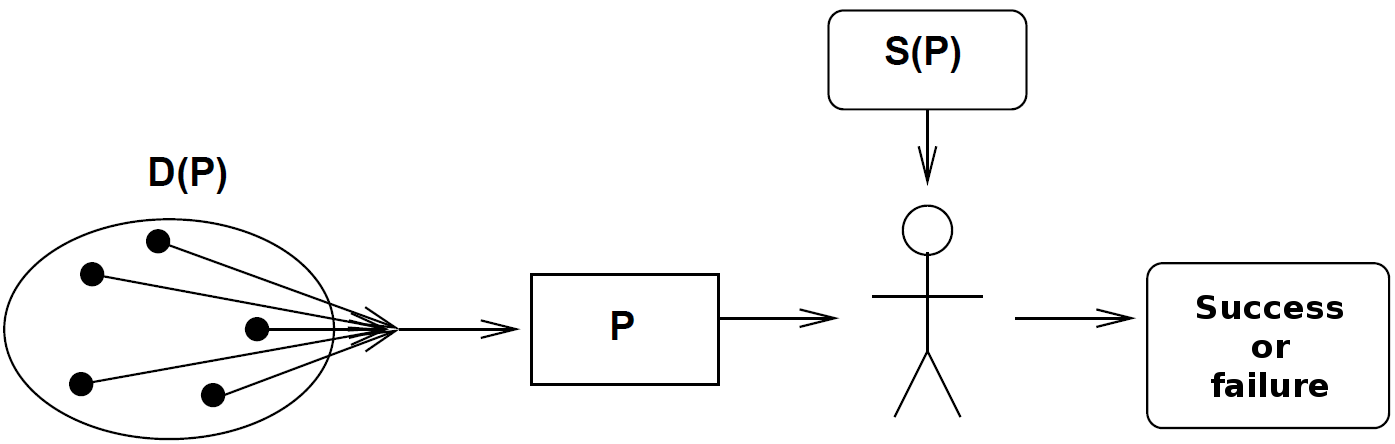
\includegraphics[width=\textwidth]{teste-de-software/conceitos-basicos/Imagens/exhaustive-software-testing}
\end{block:fact}

\hfill
\refie{example:blech-exhaustive-testing}{\beamerbutton{Example: Teste exaustivo of the blech function}}
\end{frame}



\begin{frame}
\frametitle{Técnica de teste}
\framesubtitle{Teste exaustivo}

\begin{block:fact}{Limitação do teste exaustivo}
\begin{itemize}
	\item Pode ser improveniente devivo ao tempo e ao custo de restrição, não para entrada de domínio finita, mas para grandes entradas;

	\item Impossível se o domínio de entrada é infinito;

	\item Em geral inviável.
\end{itemize}
\end{block:fact}
\end{frame}



\begin{frame}
\frametitle{Técnica de teste}
\framesubtitle{Teste aleatório}
\label{concept:random-testing}

\begin{block:concept}{Definição}
Teste aleatório utiliza um método sistemático para gerar casos de teste: requer modelar o espaço de entrada e, em seguida, os dados de amostra do espaço de entrada de forma aleatória.
\end{block:concept}

\begin{block:fact}{}
    \centering
    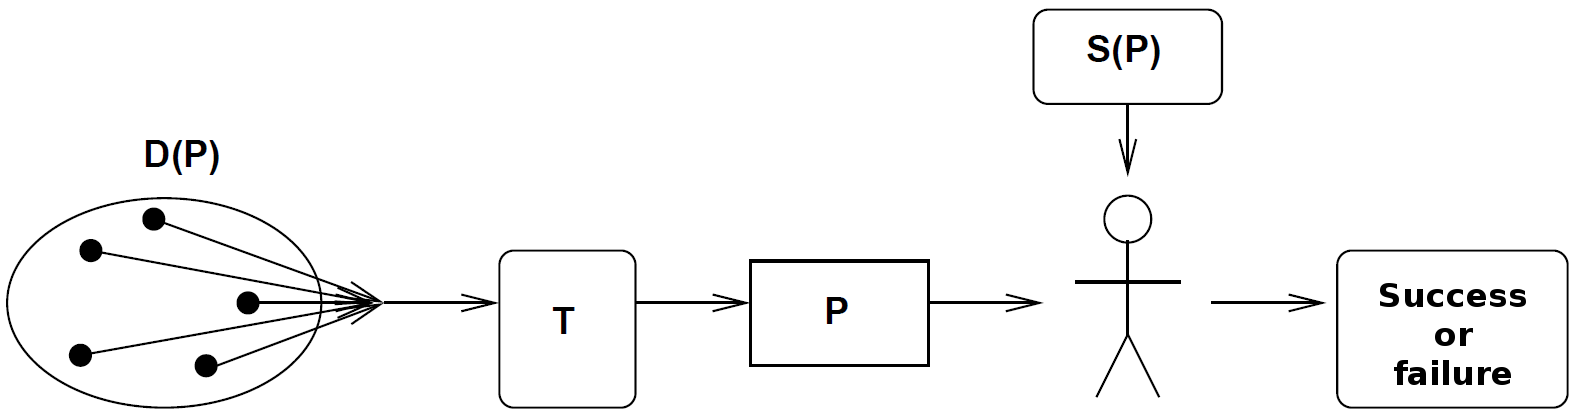
\includegraphics[width=\textwidth]{teste-de-software/conceitos-basicos/Imagens/random-software-testing}
\end{block:fact}
\end{frame}


\begin{frame}
\frametitle{Técnica de teste}
\framesubtitle{Teste aleatório}

\begin{block:concept}{Confiança}
\begin{itemize}
	\item Usando o teste aleatório, medidas estáticas de confiabilidade pode ser alcançada de acordo com um perfil operacional;

	\item Para cada (dados de entrada de um) caso de teste, é atribuída uma distribuição de probabilidade de acordo com a sua ocorrência na operação real.
\end{itemize}
\end{block:concept}

\begin{block:fact}{Eficácia}
\begin{itemize}
	\item Depende da definição do perfil operacional;

	\item Se a probabilidade de ocorrência de cada dado de entrada é o mesmo teste, o teste aleatório é considerado o teste menos eficaz para o teste de software~\cite[p. 43]{myers:2004}.
\end{itemize}

\end{block:fact}


\end{frame}


\begin{frame}
\frametitle{Técnica de teste}
\framesubtitle{Teste particionado}
\label{concept:partition-testing}

\begin{block:concept}{Definição}
Teste particionado entende-se como qualquer sistema de controle que obriga a execução de pelo menos um caso de teste a partir de cada subconjunto de uma partição do domínio de entrada.
\end{block:concept}

\begin{block:fact}{}
    \centering
    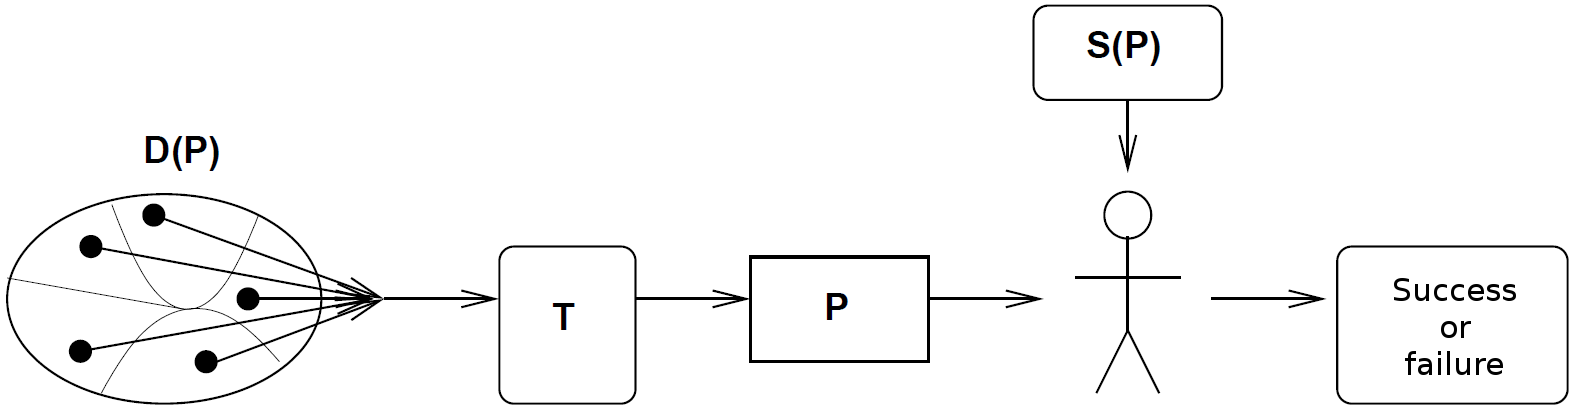
\includegraphics[width=\textwidth]{teste-de-software/conceitos-basicos/Imagens/partition-software-testing}
\end{block:fact}
\end{frame}



\begin{frame}
\frametitle{Técnica de teste}
\framesubtitle{Teste funcional}
\label{concept:functional-testing}

\begin{block:concept}{Definição}
Teste funcional é uma técnica baseada apenas nos requisitos e nas especificações.
\end{block:concept}

\begin{block:fact}{}
\begin{itemize}
	\item Teste funcional também é conhecido como teste da caixa preta;

	\item Teste funcional obtém requisitos de teste a partir da especificação de software:
	\begin{itemize}
		\item Teste funcional não requer nenhum conhecimento dos caminhos internos, a estrutura, ou a implementação do software em teste.
	\end{itemize}
\end{itemize}
\end{block:fact}

\hfill
\refie{example:functional-testing}{\beamerbutton{Example}}
\end{frame}


\begin{frame}
\frametitle{Técnica de teste}
\framesubtitle{Teste funcional}

\begin{block:fact}{Critério de teste funcional}
\begin{itemize}
	\item Partição de equivalência;
	\item Análise de valor limite;
	\item Gráfico de causa-efeito.
	\item \ldots
\end{itemize}
\end{block:fact}
\end{frame}



\begin{frame}
\frametitle{Técnica de teste}
\framesubtitle{Teste estrutural}

\begin{block:concept}{Definição}
Teste estrutural é uma técnica baseada nas partes internas, estrutura, e implementação do software em teste.
\end{block:concept}


\begin{block:fact}{}
\begin{itemize}
	\item Teste estrutural também é conhecido como caixa de teste branca;

	\item Teste estrutural consegue os requisitos de teste dos recursos de implementação.
\end{itemize}
\end{block:fact}

\begin{block:fact}{}
    \centering
    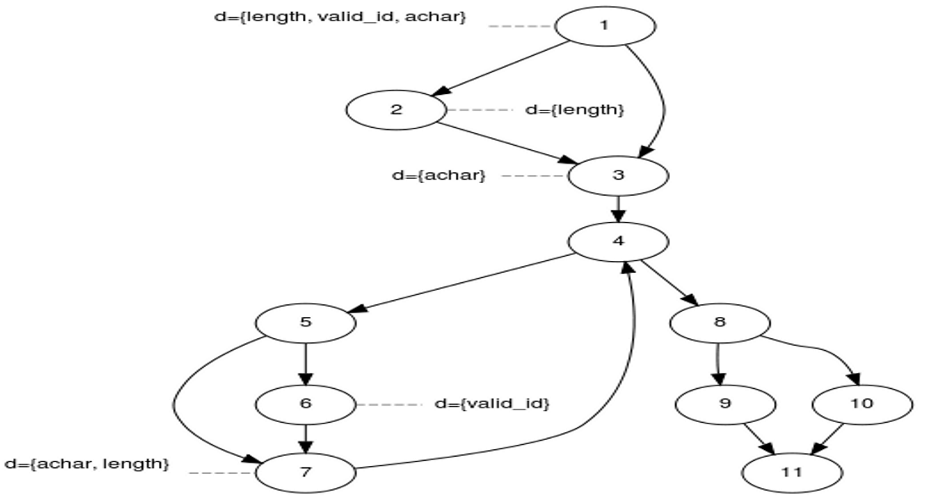
\includegraphics[width=6cm]{teste-de-software/conceitos-basicos/Imagens/structural-testing}
\end{block:fact}
\end{frame}


\begin{frame}
\frametitle{Técnica de teste}
\framesubtitle{Teste estrutural}
\label{concept:structural-testing-criteria}

\begin{block:fact}{Critérios baseados no controle de fluxo}
\begin{itemize}
	\item Critérios com base no fluxo de controle dentro de um programa:
	\begin{itemize}
		\item Cobertura de declaração;
		\item Cobertura de decisão;
		\item Cobertura de condição.
		\item \ldots
	\end{itemize}
\end{itemize}
\end{block:fact}


\begin{block:fact}{Critérios baseados no fluxo de dados}
\begin{itemize}
	\item Critérios baseados no uso de dados (criação de variável, definição e uso):
	\begin{itemize}
		\item Todas as utilizações;
		\item Todos potênciais uso;
		\item \ldots
	\end{itemize}
\end{itemize}
\end{block:fact}


\hfill
\refie{example:structural-testing}{\beamerbutton{Example}}
\end{frame}




\begin{frame}
\frametitle{Técnica de teste}
\framesubtitle{Teste baseado em erros}
\label{concept:fault-based-testing}

\begin{block:concept}{Definição}
Teste baseado em erros é uma técnica em que o teste é baseado em informações históricas sobre erros comuns detectados durante o ciclo de vida de desenvolvimento do software. 
\end{block:concept}

\begin{block:fact}{}
    \centering
    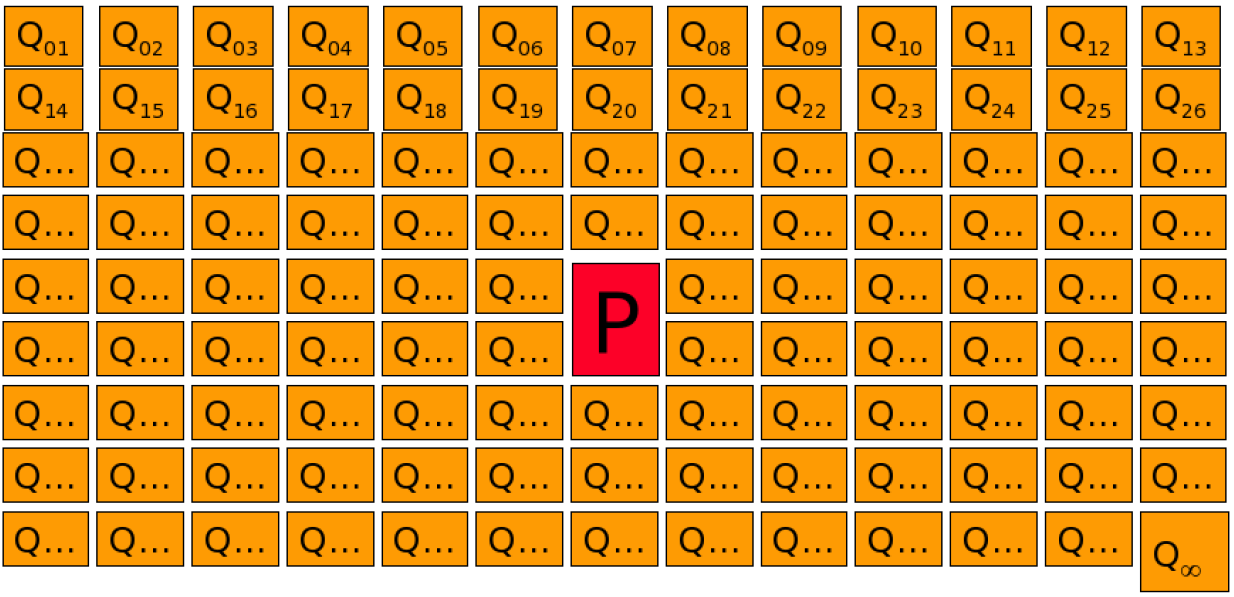
\includegraphics[width=7cm]{teste-de-software/conceitos-basicos/Imagens/mutation-testing}
\end{block:fact}
\end{frame}


\begin{frame}[hasprev=true, hasnext=false]
\frametitle{Técnica de teste}
\framesubtitle{Teste baseado em erros}
\label{concept:fault-based-test-criteria}

\begin{block:fact}{Critérios de teste baseado no erro}
\begin{itemize}
	\item Semeadura de erros.
	\item Mutação:
	\begin{itemize}
		\item Análise de mutantes;
		\item Mutação de interfaces.
		\item \ldots
	\end{itemize}
\end{itemize}
\end{block:fact}

\hfill
\refie{example:fault-based-testing}{\beamerbutton{Example}}
\end{frame} 
 
 \section{Processo de teste de software}
 \begin{frame}[parent={cmap:software-testing-foundations}, hasprev=false, hasnext=true]
\frametitle{Processo de teste de software}
\label{concept:software-testing-process}
\label{concept:test-process}

\begin{block:fact}{Processo de teste de software}
\begin{itemize}
	\item Quando realizada de forma sistemática e lúcida, o teste de software ajuda:
	\begin{itemize}
		\item Aumentar a confiança de que o produto se comporta de acordo com sua especificação;

		\item Destacar as características mínimas de qualidade do produto.
	\end{itemize}
\end{itemize}
\end{block:fact}
\end{frame}


\begin{frame}[hasprev=true, hasnext=false]
\frametitle{Conceitos de teste de software}
\framesubtitle{Teste de software}

\begin{block:fact}{}
	\centering
	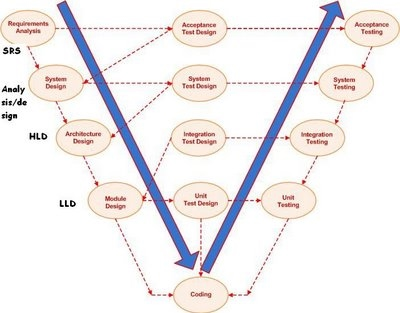
\includegraphics[width=8cm]{teste-de-software/conceitos-basicos/Imagens/v-model}
\end{block:fact}
\end{frame} 
 
 \part{Teste de software - Teste estrutural}
 
 \section{Teste estrutural}
 \begin{frame}[parent={cmap:software-testing}, hasprev=false, hasnext=true]
\frametitle{Teste estrutural}
\label{cmap:structural-software-testing}
\label{cmap:structural-testing}

\insertcmap{teste-de-software/teste-estrutural/Courses-SoftwareTesting-StructuralTesting}
\end{frame}



\begin{frame}[parent={cmap:structural-software-testing},hasnext=true,hasprev=true]
\frametitle{Teste estrutural}
\label{concept:structural-testing}

\begin{block:concept}{Definição}
Teste estrutural é uma téncnica na qual testamos baseado na parte interna, estrutura, e implementação do software em teste.
\end{block:concept}

\begin{block:fact}{Teste da caixa branca}
Como o teste estrutural deve ver os detalhes internos do software, ele também é conhecido como teste da caixa branca.
\end{block:fact}

\begin{block:fact}{Por que o teste estrutural é importante?}
\begin{itemize}
	\item O teste estrutural é muito eficiente em determinar as falhas lógicas ou de programação em fase de teste, especialmente no nivel da unidade.
\end{itemize}
\end{block:fact}
\end{frame}


\begin{frame}
\frametitle{Teste estrutural}

\begin{block:concept}{Limitações}
\begin{itemize}
	\item Teste estrutural requer habilidades de programação detalhados:
	\begin{itemize}
		\item Teste estrutural requer a intervenção do programador, a fim de determinar os caminhos inviáveis.
	\end{itemize}

	\item O número de caminhos de execução pode ser tão grande que eles não podem ser testados;

	\item Os casos de teste escolhidos podem não detectar erros de sensibilidade dos dados.
	

	\item Teste estrutural assume que o fluxo de controle está correta (ou muito perto de ser corrigida). Como os testes são baseados nos caminhos existente. Caminhos não existentes geralmente não podem ser descolbertos através desse teste estrutucal
\end{itemize}
\end{block:concept}
\end{frame}


\begin{frame}
\frametitle{Teste estrutural}

\begin{block:fact}{Quando eu posso usar o teste estrutural?}
\begin{itemize}
	\item Teste estrutural pode ser aplicado no teste unitário, integração, sistema e de fases.
\end{itemize}
\end{block:fact}


\begin{block:fact}{Teste estrutural e fases de teste}
\begin{itemize}
	\item Teste estrutural, quando aplicado na fase de teste de unidade, envolve caminhos que estão dentro de um módulo;

	\item Teste estrutural, quando aplicado na fase de teste de integração, envolve caminhos que estão entre os módulos do subsistema e caminhos entre os subsistemas dentro de sistemas;

	\item Teste estrutural, quando aplicado na fase de teste de sistema, envolve caminhos que estão entre o sistema inteiro.
	
\end{itemize}
\end{block:fact}
\end{frame}


\begin{frame}
\frametitle{Teste estrutural}

\begin{block:procedure}{Atividades de teste}
\begin{enumerate}
	\item O programa em teste em fase de implementação é analisado;
	\item Caminhos através do programa em teste são identificados;
	\item Entradas são escolhicas para fazer com que o programa em fase de teste execute o caminho selecionado. Isto é chamado de caminho de sensibilização;
	\item As saídas esperadas para essas entradas são determinadas;
	\item Os teste são executados;
	\item As saídas são comparadas com o resutado esperado, verificando se a saída real é correta.
\end{enumerate}
\end{block:procedure}
\end{frame}
 
 \section{Grafo Definição-Uso}
 \begin{frame}[parent={cmap:structural-software-testing},hasnext=true,hasprev=true]
\frametitle{Grafo definição-uso}
\label{concept:program-graph}
\label{concept:definition-use-graph}
\label{concept:dug}

\begin{block:concept}{Definição}
The Grafo Definição-Uso (DUG) é um programa gráfico adequado para representar o estado diferente de uma variável.
\end{block:concept}

\begin{block:fact}{Grafo definição-uso and grafo de fluxo de controle}
\begin{itemize}
	\item The grafo definição-uso é uma extensão do grafo de fluxo de controle;

	\item The grafo definição-uso inclui informações sobre as definições de variáveis, usos e destruições em cada nó:
	\begin{itemize}
		\item Contém todas os pares definição-uso de um programa.
	\end{itemize}
\end{itemize}
\end{block:fact}
\end{frame}


\begin{frame}
\frametitle{Grafo definição-uso}
\framesubtitle{Elementos gráficos}
\label{concept:cfg-graph-elements}

\begin{block:fact}{Elementos gráficos}
\begin{itemize}
	\item Os nós de um gráfico do programa são blocos de código indivisíveis;

	\item As extremidades do gráfico de um programa representam a possível tranferência de execução entre os blocos de código;

	\item Há somente um nó de entrada, que corresponde ao bloco de código com a primeira instrução da unidade de programa;

	\item É possível ter muitos nós de saída, isto é, sem nós de um nó seguinte.
\end{itemize}
\end{block:fact}

\hfill
\refie{example:program-graph}{\beamerbutton{Example: Program graph}}
\refie{example:identifier-cfg}{\beamerbutton{Example: Control-flow graph for Identifier}}
\end{frame}


\begin{frame}
\frametitle{Grafo definição-uso}
\framesubtitle{Blocos de código}
\label{concept:statement}
\label{concept:statement-block}
\label{concept:code-block}

\begin{block:concept}{Definição}
O bloco de código de uma programa é a sequência consecutivas de instruções com um único ponto de entrada e um único ponto de saída.
\end{block:concept}

\begin{block:fact}{Fluxo de controle e blocos de código}
\begin{itemize}
	\item Controle sempre entra em um bloco de código no seu ponto de entrada e saí no seu ponto de saída;

	\item Não há a possibilidade de saída ou uma parada em qualqer ponto dentro de um bloco de código, exceto no seu ponto de saída. 
\end{itemize}
\end{block:fact}
\end{frame}


\begin{frame}
\frametitle{Grafo definição-uso}
\framesubtitle{Blocos de código}

\begin{block:fact}{Fluxo de controle e blocos de código}
\begin{itemize}
	\item Os pontos de entrada e saída de uma bloco de código coincidem quando o bloco de código contém apenas uma declaração;

	\item Chamadas de função são frequenetemente tratados como próprios blocos de código, porque causam o controle a ser transferido distante da função atualmente em execução e, consequentemente, aumentar a possibilidade de encerramento anormal do programa.
\end{itemize}
\end{block:fact}
\end{frame}


\begin{frame}
\frametitle{Grafo definição-uso}
\framesubtitle{Decisão}
\label{concept:definition}

\begin{block:concept}{Definição}
Uma decisão é uma instrução que causa um desvio no fluxo do programa.
\end{block:concept}

\begin{block:fact}{Instruções de decisão}
\begin{itemize}
	\item A transferência de execução entre os blocos de código é uma consequência das instruções de decisão;

	\item A marioria das linguagens de alto nível fornecem instruções, como \srccode{if},
	\srccode{while} and \srccode{switch}, para servir como contexto para as decisões.
\end{itemize}
\end{block:fact}
\end{frame}


\begin{frame}
\frametitle{Grafo definição-uso}
\framesubtitle{Definição de variáveis}
\label{concept:variable-definition}

\begin{block:concept}{Definição}
Uma definição de variável é a atribuição de um valor antes de uma variável ser utilizada.
\begin{itemize}
	\item A definição de variável ocorre quando um valor é armazenado em uma posição de memória.
\end{itemize}
\end{block:concept}
\end{frame}


\begin{frame}
\frametitle{Grafo definição-uso}
\framesubtitle{Utilização de variável}
\label{concept:variable-use}

\begin{block:concept}{Definição}
A utilização de variável é quando a referência não é definida.
\end{block:concept}

\begin{block:fact}{Tipos de utilização de variável}
\begin{itemize}
	\item Há dois tipos de utilização de variável: uso computacional e uso predicativo:
	\begin{itemize}
		\item Uma variável de uso computacional (c-use) afeta diretamente o cálculo a ser efetuada ou permite que o resultado de uma definição de variável anterior seja observado;

		\item Uma variável de uso predicativo (p-use) afeta diretamente o fluxo de controle do produto em execução.
	\end{itemize}
\end{itemize}
\end{block:fact}
\end{frame}


\begin{frame}
\label{concept:dug-construction}
\frametitle{Grafo definição-uso}
\framesubtitle{Construção do Grafo definição-uso}

\begin{block:procedure}{Construção do DUG (1/2)}
\begin{enumerate}
	\item Considere um grafíco de controle de fluxo $G = (N, E)$ de um programa $P$, onde 
	$N$ é o conjunto de nós e $E$ o conjunto de extremidades. Cada nó em $G$ 
	corresponde a um bloco em $P$: aqueles blocos são denotados como 
	$b_1, b_2, ..., b_k$, addumindo que $P$ contém $k > 0$ blocos de código.

	\item Seja $def_i$ que indica o conjunto de variáveis definidas no bloco $i$.

	\item Seja $c-use_i$ que indica o conjunto de variáveis que tem um uso computacional no bloco $i$.

	\item Seja $p-use_i$ que indica o conjunto de variável que tem um uso predicativo no bloco $i$.
\end{enumerate}
\end{block:procedure}

\hfill
\refie{example:identifier-dug}{\beamerbutton{Example: Grafo definição-uso for Identifier}}
\end{frame}



\begin{frame}
\frametitle{Grafo definição-uso}
\framesubtitle{Construção do grafo definição-uso}

\begin{block:procedure}{Construção do DUG(2/2)}
\begin{enumerate}
	\setcounter{enumi}{4}
	\item Computar $def_i$, $c-use_i$, e $p-use_i$ para cada código de bloco $i$ em $P$;

	\item Associar cada nó $i$ em $N$ com $def_i$, $c-use_i$, e $p-use_i$;

	\item Para cada nó $i$ que, como um conjunto de uso predicativo não vazio e termina na 
	condição $C$, associar as extremidades $(i, j)$ e $(i, k)$ com $C$ e $!C$,
	respectivamente, dado que a extremidade $(i, j)$ é tomado quando a condição é verdadeira
	e $(i, k)$ é tomado quando a condição é falsa.
\end{enumerate}
\end{block:procedure}

\hfill
\refie{example:identifier-dug}{\beamerbutton{Example: Grafo definição-uso for Identifier}}
\end{frame}

 \section{Caminho}
 \begin{frame}[parent={cmap:structural-software-testing},hasnext=true,hasprev=true]
\frametitle{Caminho}
\label{concept:path}

\begin{block:concept}{Definição informal}
Um caminho é uma sequência de instruções.
\end{block:concept}

\begin{block:concept}{Definição}
Um caminho é uma sequência finita de nós $(n_1, n_2, . . . , nk)$,
$k \geqslant 2$, de modo que existe uma aresta de $n_i$ a $n_i + 1$ para
$i = 1, 2, ... , k - 1$.
\end{block:concept}
\end{frame}


\begin{frame}
\frametitle{Caminho}
\framesubtitle{Caminho executável e inviável}
\label{concept:infeasible-path}
\label{concept:missing-path}

\begin{block:concept}{Definição}
Um caminho executável é um caminho no qual existe um dado de entrada que pode executá-lo.
\end{block:concept}

\begin{block:concept}{Definição}
Um caminho inviável é um caminho que, para qualquer valor de entrada, não pode ser executado.
\end{block:concept}

\begin{block:fact}{Limitações e implicações}
\begin{itemize}
	\item É impossível determinar, automaticamente, caminhos inviáveis;

	\item Qualquer caminho completo que incluir um caminho inviável é um caminho inviável.
\end{itemize}
\end{block:fact}

\hfill
\refie{example:identifier-infeasible-path}{\beamerbutton{Example: Infeasible path example for Identifier}}
\end{frame}



\begin{frame}
\frametitle{Caminho}
\framesubtitle{Definition-clear path}
\label{concept:definition-clear-path}

\begin{block:concept}{Definição informal}
A caminho livre-definição é um caminho que nenhuma outra definição de variável é feita.
\end{block:concept}

\begin{block:concept}{Definição}
A caminho livre-definição com relação a uma variável $x$ é um caminho entre dois 
nós $A$ e $B$, sendo $x$ definido em $A$, com uma utilização em $B$ e com qualquer
outra definição de $x$ nos outros nós presentes no caminho entre $A$ e
$B$.
\end{block:concept}

\hfill
\refie{example:identifier-def-clear-path}{\beamerbutton{Example: Definição-clear path for Identifier}}
\end{frame}

 \section{Critério de teste de estrutura}
 \begin{frame}[parent={cmap:structural-software-testing},hasnext=true,hasprev=true]
\frametitle{Critério de teste de estrutura}
\label{concept:structural-test-criterion}

\begin{block:concept}{Definição}
Critério de teste de estrutura identifica o caminho executado dentro de uma 
unidade de progrmaa e, então, cria e executa casos de teste para cobrir esses 
caminhos, ao lado de outros requisitos de teste estabelecidos pelo Critérios 
de teste de estrutura específica.
\end{block:concept}


\begin{block:fact}{Tipos de critérios de teste de estrutura}
\begin{itemize}
	\item Há três tipos de critérios de teste de estrutura: critério de teste 
	baseado em complexidade, critério de teste de fluxo de controle, critério de teste de fluxo de dados.
\end{itemize}
\end{block:fact}

\begin{block:fact}{Teste de estrutura and JaBUTi}
\begin{itemize}
	\item JaBUTi suporta o teste de software estrural usando critérios de teste de controle de fluxo e de fluxo de dados.
\end{itemize}
\end{block:fact}
\end{frame}
 
 \section{Critério de teste de controle de fluxo}
 \begin{frame}[parent={cmap:structural-software-testing},hasnext=true,hasprev=true]
\frametitle{Critérios de teste de controle de fluxo}
\label{concept:control-flow-test-criterion}

\begin{block:concept}{Definição}
\begin{itemize}
	\item Critérios de teste de controle de fluxo emprega apenas características relacionadas
	com a estrutura de controle do programa para determinar o conjunto de requisitos
	de teste.

	\item Critérios de teste de controle de fluxo identifica os caminhos de execução
	dentro de um módulo e, em seguida, cria e executa os casos de testes para cobrir
	esses caminhos.
\end{itemize}
\end{block:concept}

\begin{block:fact}{Critérios de teste de fluxo de controle}
\begin{itemize}
	\item Todos os nós;
	\item Todas as extremidades;
	\item Todos os caminhos.
\end{itemize}
\end{block:fact}


\begin{block:fact}{Critérios de teste de fluxo de controle and JaBUTi}
\begin{itemize}
	\item Com relação ao controle de fluxo, JaBUTi suporta os seguintes critérios de teste:
	todos os nós and todas as extremidades.
\end{itemize}
\end{block:fact}
\end{frame}


\begin{frame}
\frametitle{Critérios de teste de controle de fluxo}

\begin{block:fact}{Limitações}
\begin{itemize}
	\item No critério de teste de fluxo de controle, o número de requisitos de teste
	pode ser enorme e, portanto, intestável dentro de um período razoável de tempo:
	\begin{itemize}
		\item Toda decisão que dobra o número de caminhos; cada ciclo multiplica
		os caminhos pelo número de iterações através do loop.
	\end{itemize}

	\item Os caminhos chamados na especificação pode simplesmente estar faltando em um módulo.

    \item Defeitos podem exeistir na processo de instruções sem o módulo, mesmo
	atravésdo fluxo de controle em si, é correta;

    \item O módulo pode executar corretamente para quase todos os valores de dados, mas não consegue para alguns valores.
\end{itemize}
\end{block:fact}
\end{frame}



\begin{frame}
\label{concept:all-nodes-criterion}
\label{concept:all-nodes}
\frametitle{Critérios de teste de controle de fluxo}
\framesubtitle{Todos os nós}

\begin{block:concept}{Definição}
Todos os nós requer um conjunto de teste que executa pelo menos uma vez cada nó do 
gráfico de fluxo de controle, o qual é equivalente a executar todos blocos de código de 
um programa pelo menos uma vez.
\end{block:concept}

\hfill
\refie{example:all-nodes}{\beamerbutton{Example: All-nodes example}}
\end{frame}


\begin{frame}
\frametitle{Critérios de teste de controle de fluxo}
\framesubtitle{Todos os nós}

\begin{block:fact}{Limitações}
\begin{itemize}
	\item Mesmo que o critério de todos os nós é o mais simples critério de teste 
	de estrutura, pode ser difícil satisfazer na prática:
	\begin{itemize}
		\item Muitas vezes os programas possuem códigos que é executado somente em circunstâncias
		excepcionais de pouca memória , disco cheio, arquivos ilegíveis, conexões 
		perdidas, etc;

		\item Analistas podem achar difícil ou mesmo impossível simular
		essas circunstâncias e, por conseguinte, o código que lida com esses problemas continuarão
		a serem testados.
	\end{itemize}
\end{itemize}
\end{block:fact}
\end{frame}



\begin{frame}
\label{concept:all-edges-criterion}
\label{concept:all-edges}
\frametitle{Critérios de teste de controle de fluxo}
\framesubtitle{Todas as extremidades}


\begin{block:concept}{Definição}
Todas as extremidades requer um conjunto de teste que atravessa pelo menos uma vez cada extremidade
do gráfico de fluxo de controle, isto é, o conjunto de teste assegurar que cada
instrução condicional assume valores verdadeiros e falsos, pelo menos uma vez.
\end{block:concept}
\end{frame}


\begin{frame}
\frametitle{Crtiério de teste de controle de fluxo}
\framesubtitle{Todos os caminhos}
\label{concept:all-paths-criterion}
\label{concept:all-paths}

\begin{block:concept}{Definição}
Todos os caminhos requer um conjunto de teste que executa todos os possíveos caminhos de um gráfico de controle de fluxo.
\end{block:concept}

\begin{block:fact}{Limitações}
\begin{itemize}
	\item Para unidades de programa sem laços de repetição, os requisitos de teste dos
	critérios de todos os caminhos é, em geral, pequeno o suficiente para que um caso de teste
	possa ser realmente contruído para cada caminho;

	\item Para unidades de programas com laços de repetição, os requisitos de teste para os critérios 
	de todos os caminhos pode ser enorme e, assim, apresentar um complicado problema de teste.
\end{itemize}
\end{block:fact}
\end{frame}
 
 
 \section{Critério de teste baseado em complexidade}
 \begin{frame}[parent={cmap:structural-software-testing},hasnext=true,hasprev=true]
\frametitle{Critérios de teste baseado em complexidade}
\label{concept:complexity-based-test-criterion}

\begin{block:concept}{Definição}
Critérios de teste baseado em complexidade usa informações sobre a complexidade do programa
a fim de obter os requisitos de teste
\end{block:concept}

\begin{block:fact}{Critérios de teste baseado em complexidade}
\begin{itemize}
	\item Um critério de teste baseado em complexidade bem conhecida é
	o critério de McCabe.
\end{itemize}
\end{block:fact}
\end{frame}


\begin{frame}
\label{concept:mccabe-criterion}
\frametitle{Critério baseado em complexidade}
\framesubtitle{Critérios de McCabe}

\begin{block:concept}{Definição}
O critério de McCabe requer um conjunto de caminhos completos linearmente independentes
do grafo de fluxo de controle para ser percorrido na execução do conjunto de teste.
\end{block:concept}

\begin{block:fact}{}
\begin{itemize}
	\item O critério de McCabe usa a complexidade ciclomática para obter o
	conjunto de requisitos de teste;

	\item Satisfazendo o critério de McCabe automaticamente garante tanto a
	cobertura de decição (Todas as extremidade) e cobertura de declaração (todos os nós).
\end{itemize}
\end{block:fact}
\end{frame}



\begin{frame}
\label{procedure:mccabe-criterion}
\frametitle{Critério baseado em complexidade}
\framesubtitle{Critério de McCabe}

\begin{block:procedure}{}
\begin{enumerate}
	\item Derivar o CFG do módulo de software;
	\item Computar o grafo de complexidade ciclomática (C);
	\item Selecionar um conjunto de caminhos C linearmente independentes:
	\begin{enumerate}
		\item Escolher um caminho básico (que deve ser um caminho completo):
		\begin{enumerate}
			\item Esse caminho deverá ser um caminho razoavelmente típico de execução
			ao invés de um caminho de processamento de exceção;

			\item A melhor escolha deve ser o caminho mais importante do
			ponto de vista do analista.
		\end{enumerate}

		\item Para escolher o próximo caminho, altere o resultado da primeira decição
		ao longo do caminho base, mantendo o número de outras
		decisões da mesma forma que o caminho base;

		\item Gerar o caminho remanescente através da variação das decisões restantes,
		um por um.
	\end{enumerate}
	\item Criar um caso de teste para cada caminho base.
\end{enumerate}
\end{block:procedure}


\hfill
\hyperlink{example:mccabe}{\beamerbutton{Example: McCabe's criterion example}}
\end{frame}
 

 \section{Critério de teste de fluxo de dados}
 \begin{frame}[parent={cmap:structural-software-testing},hasnext=true,hasprev=true]
\frametitle{Critério de teste de fluxo de dados}
\label{concept:data-flow-test}
\label{concept:data-flow-test-criterion}

\begin{block:concept}{Definição}
Critério de teste de fluxo de dados explora a interação envolvendo definições de
variáveis e outras referências (usos) para tais definições para estabelecer os
requisitos de teste.
\end{block:concept}


\begin{block:fact}{}
\begin{itemize}
    \item Critério de teste de fluxo de dados visa detectar falhas relacionadas com
	as definições e uso de variáveis em um programa, ou seja, o seu objetivo é o
	fluxo de dados em vez do fluxo de controle de um programa:
	\begin{itemize}
		\item Teste de fluxo de dados é uma abordagem poderosa para detectar o uso indevido
		de valores de dados devido a erro de condificação.
	\end{itemize}

	\item Critério de teste de fluxo de dados complementa o critério de teste de fluxo de controle.
\end{itemize}
\end{block:fact}
\end{frame}



\begin{frame}
\frametitle{Critério de teste de fluxo de dados}
\framesubtitle{Todas-definições}
\label{concept:all-defs}
\label{concept:all-defs-criterion}

\begin{block:concept}{Definição}
O Todas-Definições requer que uma conjunto de fluxo de dados para cada definição
de variável a ser exercida, pelo menos uma vez, por um caminho definição-limpa em
relação a c-uso ou p-uso.
\end{block:concept}
\end{frame}


\begin{frame}
\label{concept:all-uses}
\label{concept:all-uses-criterion}
\frametitle{Critério de teste de fluxo de dados}
\framesubtitle{Todos-usos}

\begin{block:concept}{Definição}
O Todos-Usos requer que todas as associações de fluxo de dados entre uma
definição de variável e todas os usos subsequentes (c-usos e p-usos) deve ser
exercido pelo menos por um caminho definição-limpa.
\end{block:concept}

\hfill
\refie{example:identifier-all-uses}{\beamerbutton{Example: All-Uses test requirements for Identifier}}

\end{frame}



\begin{frame}
\label{concept:all-p-uses}
\label{concept:all-p-uses-criterion}
\frametitle{Critério de teste de fluxo de dados}
\framesubtitle{Todos-P-Usos}

\begin{block:concept}{Definição}
O Todos-P-Usos requer que uma conjunto de fluxo de dados para cada uso
afirmativo de uma variável deve ser executada pelo menos uma vez.
\end{block:concept}
\end{frame}



\begin{frame}
\label{concept:all-c-uses}
\label{concept:all-c-uses-criterion}
\frametitle{Critério de teste de fluxo de dados}
\framesubtitle{Todos-C-Usos}

\begin{block:concept}{Definição}
O Todos-C-Usos requer que uma conjunto de fluxo de dados para cada uso
computacional de uma variável deve ser executada pelo menos uma vez.
\end{block:concept}
\end{frame}



\begin{frame}[hasnext=false]
\label{concept:all-pot-uses}
\label{concept:all-pot-uses-criterion}
\frametitle{Critério de teste de fluxo de dados}
\framesubtitle{Todos-Pot-Usos}

\begin{block:concept}{Definição}
O Todos-Pot-Usos requer para cada nó i contendo uma definição de
uma variável x que para todo nó e extremidade que possa ser alcançado a partir de i por um
caminho definição-limpa com relação a x para ser exercido.
\end{block:concept}

\hfill
\refie{example:identifier-all-pot-uses}{\beamerbutton{Example: All-Potential-Uses test requirements for Identifier}}
\end{frame}  
 
 \part{Referências e créditos}
 
 \section{Referências}
 \begin{frame}
  \frametitle{Referências}
  \begin{itemize}
    \item Site das maratonas
    \begin{itemize}
      \item \url{http://icpc.baylor.edu/}
      \item \url{http://maratona.ime.usp.br/}
    \end{itemize}
    \item Site de simulação dos problemas
    \begin{itemize}
      \item \url{http://br.spoj.com/}
      \item \url{http://uva.onlinejudge.org/}
      \item \url{www.urionlinejudge.com.br}
      \item \url{www.programming-challenges.com}
    \end{itemize}
  \end{itemize}
\end{frame}
 
 \section{Bibliografia}
 \part{References}
\section*{References}

\nocite{ammann-offutt:2008}
\nocite{mathur:2008}

\begin{frame}[label=references, allowframebreaks]{\refname}
\bibliographystyle{abnt-num}
\bibliography{Competitive_Programming_3}
\end{frame}
 
%  \section{Créditos}
%  \begin{frame}[c,label=credits]
  \frametitle{Cr�ditos}

  \begin{itemize}
    \item Reviewers:
    \begin{itemize}
      % \item Auri Marcelo Rizzo Vincenzi
      % \item Ellen Francine Barbosa
      \item Fabiano Cutigi Ferrari
      % \item M�rcio Eduardo Delamaro
      \item Ot�vio Augusto Lazzarini Lemos
    \end{itemize}
  \end{itemize}
\end{frame}

\end{document}
